\newpage

\subsection{Methyl 3-oxodecanoate \compound{cmpd:bke}}

%lit
%LMO-1-034
\begin{scheme}[H]
	\begin{center}
		\schemeref[bke]{cmpd:bke}
		\schemeref[bket]{cmpd:bket}
		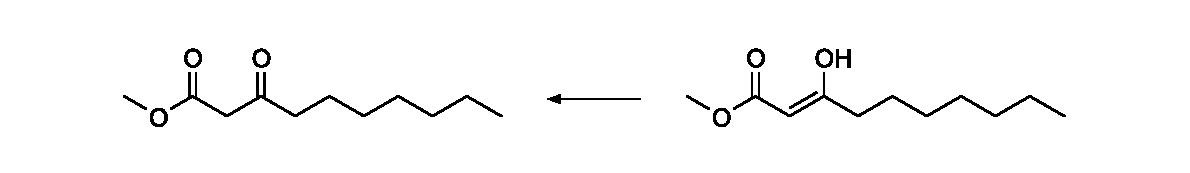
\includegraphics[scale=1]{bke}
	\end{center}
\end{scheme}

Meldrum's acid \compound{cmpd:Mel} (9.00 g, 63.0 mmol, 1 eq.)\ was dissolved in anhydrous \ce{CH2Cl2} (150 mL) in an oven-dried flask and cooled to $0\ ^{\circ}$C. Pyridine (10.2 mL, 126 mmol, 2 eq.) was added dropwise over 20 min. Octanoyl chloride \compound{cmpd:OctoCl} (11.7 mL, 69.0 mmol, 1.1 eq.)\ was then added and the mixture was stirred at $0\ ^{\circ}$C for a further 4 h. 
The mixture was allowed to warm to r.t., diluted with \ce{CH2Cl2} (20 mL) and poured into a mixture of ice (\textasciitilde 30 g) and HCl (2 N, 90 mL). The solution was washed with NaCl (sat., aq., 150 mL) and dried over \ce{MgSO4}. The solvent was removed under vacuum to give an orange-brown oil.
The oil was refluxed in anhydrous MeOH (150 mL) for 5 h and the solvent was removed under vacuum. The resulting residue was purified by column chromatography (\ce{SiO2}, 5\% \ce{Et2O}/40-60 P.E.). A tautomeric mixture of \compound{cmpd:bke} and \compound{cmpd:bket} was obtained as a colourless oil (8.34 g, 41.6 mmol, 66\%. 92\% \compound{cmpd:bke} as determined by $^{1}$H NMR).

\subsubsection*{Keto form \compound{cmpd:bke}}%\\[1\baselineskip]
\noindent{\textbf{TLC} \textit{R$_f$} = 0.12 (5\% \ce{EtO2}/PE)}
\\[1\baselineskip]
\noindent{\textbf{IR} (neat) $\nu_{max}$ / cm$^{-1}$ = 
	2928 (C-H),
	2856 (C-H),
	1747 (ester C=O),
	1717	(ketone C=O)}
\\[1\baselineskip]
\textbf{$^{1}$H NMR} (400 MHz, CDCl$_3$) $\delta$ / ppm = 
	3.74 (s, 3 H, OC\underline{H}$_3$), 
	3.45 (s, 2 H, C(=O)C\underline{H}$_2$C(=O)), 
	2.53 (t, \textit{J} = 7.4 Hz, 2 H, C(=O)C\underline{H}$_2$CH$_2$), 
	1.60 (quin, \textit{J} = 7.1 Hz, 2 H, C(=O)CH$_2$C\underline{H}$_2$),
	1.39 - 1.19 (m, 8 H, C\underline{H}$_2$C\underline{H}$_2$C\underline{H}$_2$C\underline{H}$_2$CH$_3$), 
	0.88 (t, \textit{J} = 6.8 Hz, 3 H, CH$_2$C\underline{H}$_3$)
\\[1\baselineskip]
\textbf{$^{13}$C NMR} (101 MHz, CDCl$_3$) $\delta$ / ppm = 
	202.3 (CH$_3$OC(=O)CH$_2$\underline{C}(=O)), 
	167.3 (CH$_3$O\underline{C}(=O)CH$_2$C(=O)),
	51.7 (O\underline{C}H$_3$), 
	48.5 (CH$_3$OC(=O)\underline{C}H$_2$C(=O)), 
	42.5 (C(=O)\underline{C}H$_2$CH$_2$), 
	31.3 (\underline{C}H$_2$), 
	28.7 (\underline{C}H$_2$), 
	28.6 (\underline{C}H$_2$), 
	23.1 (\underline{C}H$_2$), 
	22.2 (\underline{C}H$_2$), 
	13.6 (CH$_2$\underline{C}H$_3$)
	%42.5 (\underline{C}H$_2$CH$_2$CH$_2$CH$_2$CH$_2$CH$_2$CH$_3$), 
	%31.3 (CH$_2$\underline{C}H$_2$CH$_2$CH$_2$CH$_2$\-CH$_2$\-CH$_3$), 
	%28.7 (CH$_2$CH$_2$\underline{C}H$_2$CH$_2$\-CH$_2$\-CH$_2$CH$_3$), 
	%28.6 (CH$_2$CH$_2$CH$_2$\underline{C}H$_2$CH$_2$CH$_2$CH$_3$), 
	%23.1 (CH$_2$CH$_2$CH$_2$CH$_2$\-\underline{C}H$_2$CH$_2$CH$_3$), 
	%22.2 (CH$_2$CH$_2$CH$_2$CH$_2$CH$_2$\underline{C}H$_2$CH$_3$),  
	%13.6 (CH$_2$CH$_2$CH$_2$CH$_2$CH$_2$CH$_2$\underline{C}H$_3$)

\subsubsection*{Enol form \compound{cmpd:bket}}
\noindent{\textbf{TLC} \textit{R$_f$} = 0.12 (5\% \ce{EtO2}/PE)}
\\[1\baselineskip]
\noindent{\textbf{IR} (neat) $\nu_{max}$ / cm$^{-1}$ = 
	2928 (C-H),
	2856 (C-H),
	1654	(C=C),
	1629 ($\alpha$,$\beta$ unsaturated C=O)}
\\[1\baselineskip]
\textbf{$^{1}$H NMR} (400 MHz, CDCl$_3$) $\delta$ / ppm = 
	12.02 (s, 1 H, CO\underline{H}), 
	4.99 (s, 1 H, C(=O)C\underline{H}=COH),
	3.73 (s, 3 H, OC\underline{H}$_3$), 
	2.20 (t, \textit{J} = 7.4 Hz, 2 H, COHC\underline{H}$_2$), 
	1.76 - 1.72 (m, 2 H, COHCH$_2$C\underline{H}$_2$),
	1.39 - 1.19 (m, 8 H, C\underline{H}$_2$C\underline{H}$_2$C\underline{H}$_2$C\underline{H}$_2$CH$_3$), 
	0.88 (t, \textit{J} = 6.8 Hz, 3 H, CH$_2$C\underline{H}$_3$)
	\\[1\baselineskip]
\textbf{$^{13}$C NMR} (101 MHz, CDCl$_3$) $\delta$ / ppm = 
	178.7 (CH$_3$OC(=O)CH=\underline{C}OH), 
	172.7 (CH$_3$O\underline{C}(=O)CH=COH), 
	88.2 (CH$_3$OC\-(=O)\underline{C}H=COH), 
	50.5 (O\underline{C}H$_3$),
	37.9 (COH\underline{C}H$_2$CH$_2$), 
	34.6 (\underline{C}H$_2$), 
	31.2 (\underline{C}H$_2$), 
	29.0 (\underline{C}H$_2$), 
	25.9 (\underline{C}H$_2$), 
	22.3 (\underline{C}H$_2$), 
	13.6 (CH$_2$\underline{C}H$_3$)
	%37.9 (\underline{C}H$_2$CH$_2$CH$_2$CH$_2$CH$_2$CH$_2$CH$_3$), 
	%34.6 (CH$_2$\underline{C}H$_2$CH$_2$CH$_2$CH$_2$\-CH$_2$\-CH$_3$), 
	%31.2 (CH$_2$CH$_2$\underline{C}H$_2$CH$_2$\-CH$_2$CH$_2$CH$_3$), 
	%29.0 (CH$_2$CH$_2$CH$_2$\underline{C}H$_2$CH$_2$CH$_2$CH$_3$), 
	%25.9 (CH$_2$CH$_2$CH$_2$CH$_2$\-\underline{C}H$_2$\-CH$_2$\-CH$_3$), 
	%22.3 (CH$_2$CH$_2$CH$_2$\-CH$_2$CH$_2$\underline{C}H$_2$CH$_3$), 
	%13.6 (CH$_2$CH$_2$CH$_2$CH$_2$CH$_2$CH$_2$\underline{C}H$_3$)}
\\[1\baselineskip]
Spectroscopic data are consistent with the literature\cite{Baker2012,Scribner1978}.
%lit

%Enol
%δH (400 MHz, CDCl3): 11.98 (1H, s, COCHCOH), 4.95 (1H, s, COCHCOH), 3.70 (3H, s, CH3OCO), 2.15 (2H, t, \textit{J}=7.6 Hz, CHCOHCH2), 1.72-1.68 (2H, m, COHCH2CH2), 1.34-1.20 (8H, m, CH2CH2CH2CH2CH3), 0.84 (3H, t, \textit{J}=6.9 Hz, CH2CH3);
%δC (101 MHz, CDCl3): 179.2 (COCHCOH), 170.0 (CH3OCO), 101.8 (COCHCOH), 51.7 (CH3O), 38.41 (COCH2CH2), 35.1 (CH2), 33.6 (CH2), 29.8 (CH2), 26.3 (CH2), 23.9 (CH2), 14.5 (CH2CH3).
%Keto form:
%δH (400 MHz, CDCl3): 3.70 (3H, s, CH3OCO), 3.41 (2H, s, COCH2CO), 2.51 (2H, t, \textit{J}= 7.4 Hz, COCH2COCH2), 1.59-1.52 (2H, m, COCH2CH2), 1.34-1.20 (8H, m, CH2CH2CH2CH2CH3), 0.84 (3H, t, \textit{J} = 6.9 Hz, CH2CH3);
%δC (101 MHz, CDCl3): 203.0 (CH2COCH2), 167.8 (CO2Me), 52.4 (CH3O), 49.1 (COCH2CO), 43.1 (COCH2CH2), 31.7 (CH2), 29.2 (CH2), 29.0 (CH2), 23.5 (CH2), 22.6 (CH2), 14.1 (CH2CH3).

%\subsection{Methyl (E)-3-((4-aminophenyl)amino)dec-2-enoate \compound{cmpd:enaman}}
%
%%Yssymaking
%
%\begin{scheme}[H]
%	\begin{center}
%		\includegraphics[scale=1]{enaman}
%	\end{center}
%\end{scheme}

\subsection{Methyl (\textit{E})-3-((4-((\textit{tert}-butoxycarbonyl)amino)phenyl)amino)dec-2-enoate \compound{cmpd:Bocenaman}}

%LMO-1-061

\begin{scheme}[H]
	\begin{center}
		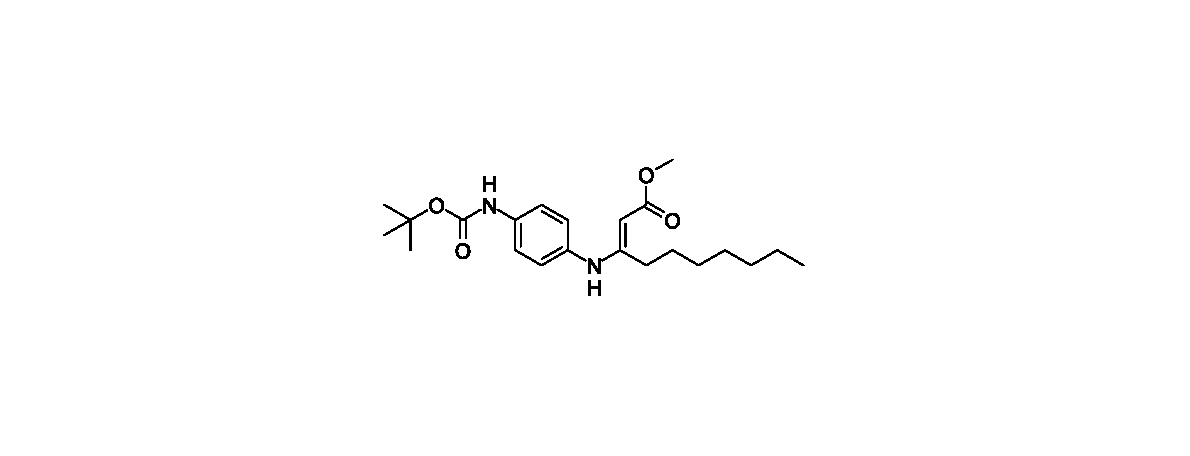
\includegraphics[scale=1]{Bocenaman}
	\end{center}
\end{scheme}

Methyl 3-oxodecanoate \compound{cmpd:bke} (500 mg, 2.50 mmol, 1.00 eq.) and \textit{O}-\textit{tert}-butyl \textit{N}-(4-aminophenyl)carbamate \compound{cmpd:ambenboc} (520 mg, 2.50 mmol, 1.00 eq.) were dissolved in MeOH (10 mL) and refluxed for 18 h. The solvent was removed under vacuum and the resulting residue was purified by column chromatography (\ce{SiO2}, gradient of 0 to 20\% \ce{Et2O}/40-60 P.E.). \compound{cmpd:Bocenaman} was obtained as a white amorphous solid (0.169 mg, 0.480 mmol, 19\%).
\\[1\baselineskip]
\noindent{\textbf{TLC} \textit{R$_f$} = 0.30 (30\% \ce{Et2O}/40-60 P.E.)}
\\[1\baselineskip]
\noindent{\textbf{mp} \textit{T} / $^{\circ}$C = 79 (\ce{Et2O}/40-60 P.E.)}
\\[1\baselineskip]
\noindent{\textbf{IR} (neat) $\nu_{max}$ / cm$^{-1}$ = 
	3337 (N-H),
	2928 (C-H),
	2857 (C-H),
	1724 (carbamate C=O),
	1635 ($\alpha$,$\beta$ unsaturated C=O),
	1611 (C=C),
	1581 (N-H bend)}
\\[1\baselineskip]
\noindent{\textbf{$^{1}$H NMR} (400 MHz, CDCl$_3$) $\delta$ / ppm = 
10.16 (s, 1 H, N\underline{H}C(C$_{7}$H$_{15}$)=C), 
7.35 (d, \textit{J} = 8.6 Hz, 2 H, \textit{meta} to NHBoc), 
7.02 (d, \textit{J} = 8.7 Hz, 2 H, \textit{meta} to enamine), 
6.60 (br s, 1 H, N\underline{H}Boc), 
4.71 (s, 1 H, C=C\underline{H}), 
3.70 (s, 3 H, OC\underline{H}$_3$), 
2.23 (t, \textit{J} = 7.7 Hz, 2 H, C\underline{H}$_2$CH$_2$CH$_2$CH$_2$CH$_2$CH$_2$CH$_3$), 
1.54 (s, 9 H, C(C\underline{H}$_3$)$_3$), 
1.40 (quin, \textit{J} = 7.3 Hz, 2 H, CH$_2$C\underline{H}$_2$CH$_2$CH$_2$CH$_2$CH$_2$CH$_3$), 
1.33 - 1.16 (m, 8 H, CH$_2$CH$_2$C\underline{H}$_2$C\underline{H}$_2$C\underline{H}$_2$C\underline{H}$_2$CH$_3$), 
0.86 (t, \textit{J} = 7.1 Hz, 3 H, CH$_2$CH$_2$CH$_2$CH$_2$CH$_2$CH$_2$C\underline{H}$_3$)
\\[1\baselineskip]
\textbf{$^{13}$C NMR} (101 MHz, CDCl$_3$) $\delta$ / ppm = 
171.1 (\underline{C}(=O)CH=C), 
164.3 (C(=O)CH=\underline{C}), 
152.7 (O\underline{C}(=O)NH), 
136.0 (\textit{para} to NHBoc), 
134.1 (\underline{C}NHBoc), 
126.3 (\textit{meta} to NHBoc), 
119.1 (\textit{ortho} to NHBoc), 
83.8 (C(=O)\underline{C}H=C), 
80.7 (\underline{C}(CH$_3$)$_3$), 
50.2 (O\underline{C}H$_3$), 
32.2 (\underline{C}H$_2$), 
31.6 (\underline{C}H$_2$), 
29.1 (\underline{C}H$_2$), 
28.8 (\underline{C}H$_2$), 
28.3 (C(\underline{C}H$_3$)$_3$), 
28.0 (\underline{C}H$_2$), 
22.6 (\underline{C}H$_2$), 
14.0 (\underline{C}H$_3$)}
\\[1\baselineskip]
\noindent{\textbf{HRMS} (ESI$^+$) \textit{m}/\textit{z} / Da = 391.2589, [M+H]$^+$, [\ce{C22H35N2O4}]$^+$ requires 391.2591}
\\[1\baselineskip]
Spectroscopic data are consistent with the literature\cite{Baker2015}.

%Rf : 0.45 (30% Et2O/hexane); δH (500 MHz, CDCl3 ): 10.15 (1H, s, H12), 7.33 (2H, d, J
%= 8.5 Hz, H15), 7.02 (2H, d, J = 8.7 Hz, H14), 6.48 (1H, s, H17), 4.69 (1H, s, H2), 3.68 (3H, s, H11), 2.21 (2H, t, J = 7.8 Hz, H4), 1.52 (9H, s, H20), 1.28 (10H, m, H5- H9), 1.41-1.15 (3H t, J = 7.2 Hz, H10); δC
%(126 MHz, CDCl3 ): 171.2 (C1), 164.4
%(C3), 152.8 (C18), 136.1 (C13), 134.3 (C16), 126.4 (C15), 119.2 (C14), 84.0 (C2), 80.9 (C19), 50.4 (C11), 32.3 (C4), 31.7 (C5), 29.2 (C6, C7 or C8), 28.9 (C6, C7 or C8), 28.5 (C20), 28.1 (C6, C7 or C8), 22.7 (C9), 14.2 (C10); νmax
%(neat)/cm-1 : 3340
%(m, N-H), 3259 (m, N-H), 2939 (m, C-H), 1724 (s, C=O ester), 1634 (s, C=O), 1610 (m, C=C), 1583 (MC=C), 1519 (S, C=C); HRMS (ESI+) calculated for C22
%H35 N2 O4 [M+H]+ : 391.2587; found: 391.2587.

%SM
%1,2-Diamino-N-(tert-butyloxycarbonyl)benzene (14): 1,2-Diaminobenzene (2.5 g, 25 mmol) and Boc-ON (6.15 g, 25 mmol) were dissolved in DMF (50 mL) and heated to 55 °C for 3 h. The solvent was removed in vacuo and the residue dissolved in toluene (60 mL). The organic layer was washed with aqueous NaOH (10 %, 2×50 mL) and NaCl (10 %, 2×50 mL) and dried with MgSO4. Recrystallisation from chloroform/hexane gave a colourless powder. Yield: 3.0 g (15.8 mmol, 63 %). 1H NMR (300 MHz, CDCl3): δ=7.43 (dd, 1 H; Ar-H), 7.15 (td, 1 H; Ar-H), 6.93 (td, 1 H; Ar-H), 6.89 (dd, 1 H; Ar-H), 6.61 (s, 1 H; C(O)NH), 3.88 (s, 2 H; NH2), 1.69 ppm (s, 9 H; CH3); 13C NMR (75 MHz, CDCl3): δ=153.8 (C(O)NH), 139.9, 125.9, 124.7, 124.6, 119.3, 117.3 (Ar-C), 80.3 (OC(CH3)3), 28.2 ppm (OC(CH3)3); MS (70 eV): \textit{m}/\textit{z} / Da (%) 208 (53) [M+], 152 (99) [M+−tBu], 135 (38) [M+−OtBu], 108 (100) [M+−Boc]; elemental analysis calcd (%) for C11H16N2O2: C 63.44, H 7.74, N 13.45; found: C 63.30, H 7.61, N 13.34.

\subsection{6-Amino-2-heptylquinolin-4-ol \compound{cmpd:amHHQ}}
%LMO-1-062

\begin{scheme}[H]
	\begin{center}
		\includegraphics[scale=1]{amHHQ}
	\end{center}
\end{scheme}

Methyl (\textit{E})-3-((4-((\textit{tert}-butoxycarbonyl)amino)phenyl)amino)dec-2-enoate \compound{cmpd:Bocenaman} (168 mg, 0.649 mmol, 1 eq.) and polyphosphoric acid (5 g) were heated to $90\ ^{\circ}$C for 1 h. The reaction mixture was then poured into \ce{NaHCO3} (sat., aq., 50 mL) cooled with ice. The precipitate was collected by vacuum filtration, washed with water (50 mL) and dried under high vacuum. \compound{cmpd:amHHQ} was obtained as a pale yellow amorphous solid (121 mg, 0.468 mmol, 72\%).
\\[1\baselineskip]
\noindent{\textbf{mp} \textit{T} / $^{\circ}$C = 249 (water)}
\\[1\baselineskip]
\noindent{\textbf{IR} (neat) $\nu_{max}$ / cm$^{-1}$ = 
	3337 (N-H),
	2927 (C-H),
	2857 (C-H),
	%1724 (C=O),
	1635 (C=O)}
	%1611 (aromatic),
	%1583 (aromatic),
	%1519 (aromatic)}
\\[1\baselineskip]
\noindent{\textbf{$^{1}$H NMR} (400 MHz, DMSO-d$_6$) $\delta$ / ppm = 
	7.26 (d, \textit{J} = 8.7 Hz, 1 H, \textit{meta} to NH$_2$), 
	7.15 (d, \textit{J} = 2.6 Hz, 1 H, \textit{ortho} to C(=O)), 
	6.95 (dd, \textit{J} = 2.7, 8.8 Hz, 1 H, \textit{para} to C(=O)), 
	5.74 (s, 1 H, \textit{ortho} to CH$_2$), 
	5.16 (s, 2 H, N\underline{H}$_2$), 
	2.52 (t, \textit{J} = 7.4 Hz, 2 H, CC\underline{H}$_2$), 
	1.64 (quin, \textit{J} = 7.6 Hz, 2 H, CCH$_2$C\underline{H}$_2$), 
	1.36 - 1.19 (m, 8 H, C\underline{H}$_2$C\underline{H}$_2$C\underline{H}$_2$C\underline{H}$_2$CH$_3$), 
	0.86 (t, \textit{J} = 7.0 Hz, 3 H, \underline{H}$_3$)
\\[1\baselineskip]
\textbf{$^{13}$C NMR} (101 MHz, DMSO-d$_6$) $\delta$ / ppm = 
	176.7 (\underline{C}(=O)), 
	151.7 (\underline{C}CH$_2$), 
	145.1 (\textit{para} to NH$_2$ or \textit{ipso} to C(=O)), 
	132.4 (\textit{ipso} to NH$_2$), 
	126.6 (\textit{para} to NH$_2$ or \textit{ipso} to C(=O)), 
	121.1 (\textit{para} to C(=O)), 
	119.0 (\textit{meta} to NH$_2$ and \textit{meta} to C(=O)), 
	106.2 (\underline{C}H=CCH$_2$), 
	105.9 (\textit{ortho} to NH$_2$ and \textit{ortho} to C(=O)), 
	33.6 (C\underline{C}H$_2$), 
	31.6 (\underline{C}H$_2$CH$_2$CH$_3$), 
	29.0 (\underline{C}H$_2$), 
	29.0 (\underline{C}H$_2$), 
	28.9 (\underline{C}H$_2$), 
	22.5 (\underline{C}H$_2$CH$_3$), 
	14.4 (\underline{C}H$_3$)}
\\[1\baselineskip]
\noindent{\textbf{HRMS} (ESI$^+$) \textit{m}/\textit{z} / Da = 259.1810, [M+H]$^+$, [\ce{C16H23N2O}]$^+$ requires 259.1803}
\\[1\baselineskip]
Spectroscopic data are consistent with the literature\cite{Baker2015}.
%rough

\subsection{6-Azido-2-heptylquinolin-4-ol \compound{cmpd:azHHQ}}
%LMO-1-067

\begin{scheme}[H]
	\begin{center}
		\includegraphics[scale=1]{azHHQ}
	\end{center}
\end{scheme}

6-Amino-2-heptylquinolin-4-ol \compound{cmpd:amHHQ} (50 mg, 0.194 mmol, 1 eq) was dissolved in HCl (conc., aq., 1.20 mL), water (1.80 mL) and MeOH (2.00 mL) and cooled to 0 $^{\circ}$C. A solution of \ce{NaNO2} (16.0 mg, 0.232 mmol, 1.2 eq.) in water (0.300 mL) was added dropwise over 10 min and the mixture was stirred for 1 h. A solution of \ce{NaN3} (15.1 mg, 0.232 mmol, 1.2 eq.) in water (0.300 mL) was then added. The mixture was warmed to room temperature and stirred for a further 4 h. The resultant precipitate was filtered off and dried under reduced pressure. \compound{cmpd:azHHQ} hydrochloride salt* was obtained as a pale cream amorphous solid (25.6 mg, 0.0800 mmol, 41\%).
\\[1\baselineskip]
\noindent{\textbf{TLC} \textit{R$_f$} = 0.40 (5\% MeOH/\ce{CH2Cl2})}
\\[1\baselineskip]
%\noindent{\textbf{mp} \textit{T} / $^{\circ}$C = ?? (??)}
%\\[1\baselineskip]
\noindent{\textbf{IR} (neat) $\nu_{max}$ / cm$^{-1}$ = 
	3249 (N-H),
	3065 (N-H),
	2917 (C-H),
	2853 (C-H),
	2728 (C-H),
	2107 (azide),
	1635 (C=O)} 
\\[1\baselineskip]
\noindent{\textbf{$^{1}$H NMR} (400 MHz, MeOD) $\delta$ / ppm = 
	7.73 (d, \textit{J} = 8.6 Hz, 1 H, \textit{ortho} to NH), 
	7.71 (d, \textit{J} = 2.8 Hz, 1 H, \textit{ortho} to N$_3$ and \textit{ortho} to C(=O)), 
	7.47 (dd, \textit{J} = 8.9, 2.7 Hz, 1 H, \textit{para} to C(=O)), 
	6.24 (s, 1 H, C(=O)C\underline{H}), 
	2.69 (t, \textit{J} = 7.7 Hz, 2 H, CC\underline{H}$_2$), 
	1.68 (quin, \textit{J} = 7.6 Hz, 2 H, CCH$_2$C\underline{H}$_2$), 
	1.28 - 1.39 (m, 4 H, CCH$_2$CH$_2$C\underline{H}$_2$C\underline{H}$_2$), 
	1.18 - 1.28 (m, 4 H, C\underline{H}$_2$C\underline{H}$_2$CH$_3$), 
	0.85 (t, \textit{J} = 6.8 Hz, 3 H, C\underline{H}$_3$)}
\\[1\baselineskip]
\noindent{\textbf{$^{13}$C NMR} (101 MHz, MeOD) $\delta$ / ppm = 
	172.3 (\underline{C}(=O)), 
	155.5 (NH\underline{C}CH$_2$), 
	137.4 (\underline{C}N$_3$), 
	135.6 (\textit{para} to N$_3$), 
	124.6 (\textit{para} to C(=O)), 
	124.1 (\textit{ipso} to C(=O)), 
	120.7 (\textit{meta} to N$_3$ and \textit{meta} to C(=O)), 
	112.8 (\textit{ortho} to N$_3$ and \textit{ortho} to C(=O)), 
	107.0 (C(=O)\underline{C}H), 
	33.3 (NHC\underline{C}H$_2$), 
	31.2 (\underline{C}H$_2$CH$_2$CH$_3$), 
	28.3 - 28.5 (\underline{C}H$_2$\underline{C}H$_2$\underline{C}H$_2$CH$_2$CH$_2$CH$_3$), 
	22.1 (\underline{C}H$_2$CH$_3$), 
	14.0 (\underline{C}H$_3$)}
\\[1\baselineskip]
\noindent{\textbf{HRMS} (ESI$^+$) \textit{m}/\textit{z} / Da = 285.1728, [M+H]$^+$ found, [\ce{C16H21N4O}]$^+$ requires 285.1715
\\[1\baselineskip]
Spectroscopic data are similar to the literature characterisation of the free amine\cite{Baker2015}.

\noindent{*Probably as the 4-hydroxyquinoline\cite{Hodgkinson2011}.}

\subsection{Heptyl magnesium bromide \compound{cmpd:hepGr}}

%lit

\begin{scheme}[H]
	\begin{center}
		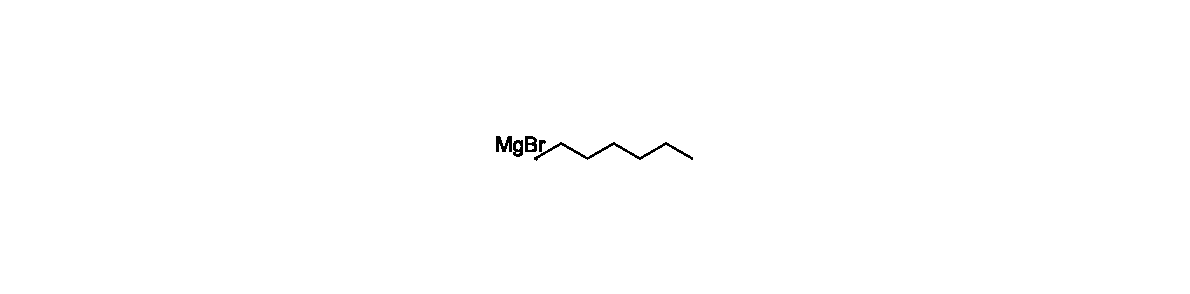
\includegraphics[scale=1]{hepGr}
	\end{center}
\end{scheme}

Magnesium turnings (352 mg, 14.5 mmol, 1 eq.) were added to an oven-dried flask under argon. THF (15 mL) was added, followed by bromoheptane \compound{cmpd:hepBr} (2.40 mL, 14.5 mmol, 1 eq.) dropwise. The mixture was stirred at r.t. for 2 h followed by heating to reflux for 2 h. Heptyl magnesium bromide \compound{cmpd:hepGr} was obtained as a pale grey suspension (15 mL, \textasciitilde ~1 M) which was used without further purification.

\subsection{2-Chloro-\textit{N}-methoxy-\textit{N}-methylacetamide \compound{cmpd:ClWa}}

\begin{scheme}[H]
	\begin{center}
		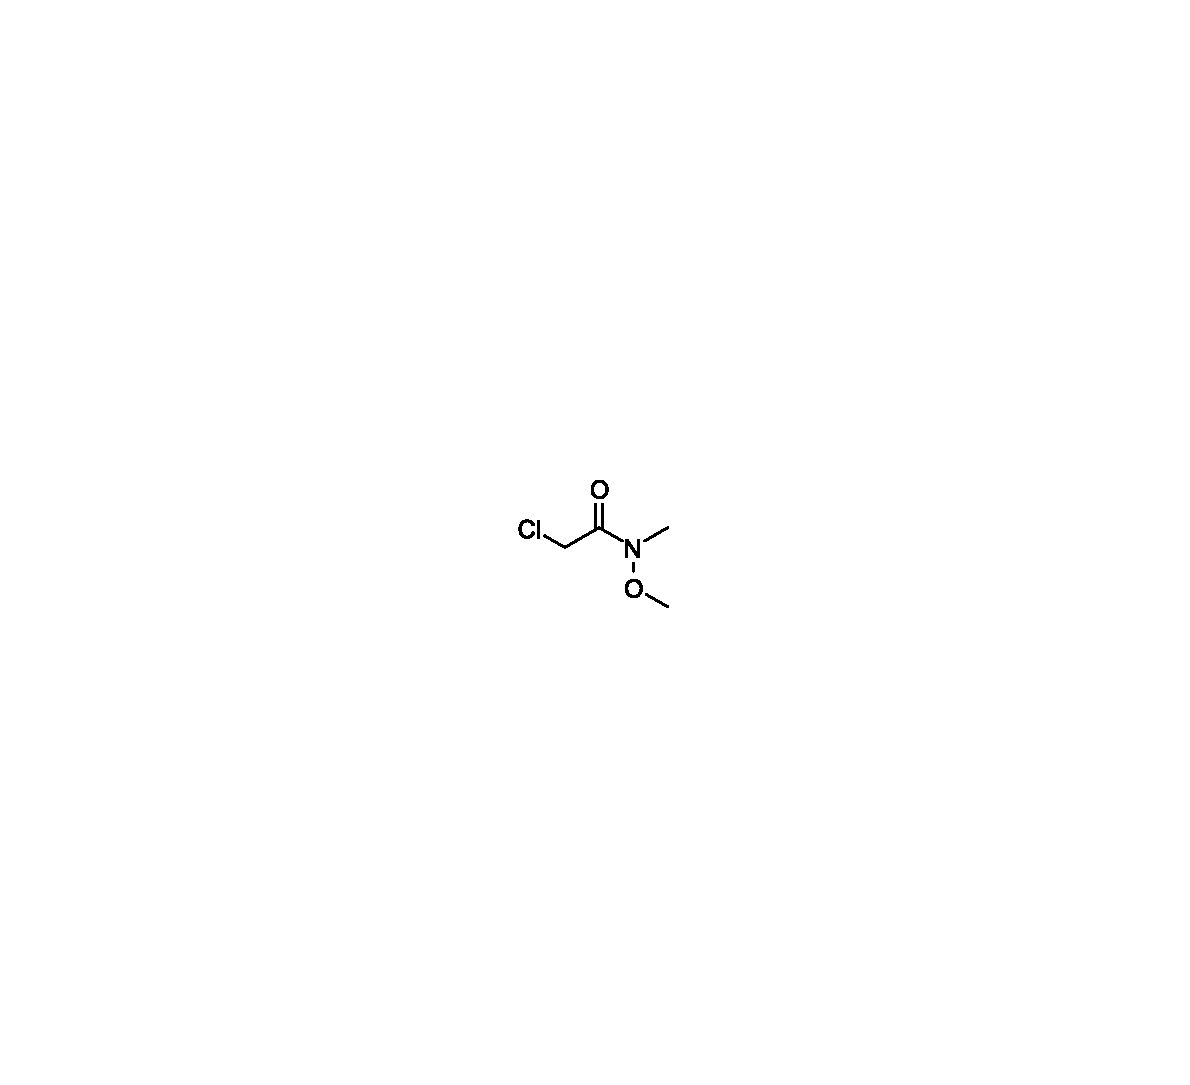
\includegraphics[scale=1]{ClWa}
	\end{center}
\end{scheme}

%lit

\textit{N},\textit{O}-Dimethylhydroxyl amine hydrochloride \compound{cmpd:DMHAHCl} (6.00 g, 61.5 mmol, 1 eq.) and toluene (75 mL) were 
added successively to a stirred solution of potassium carbonate (22.4 g, 162 mmol, 2.63 eq.) in water (75 mL) at $0\ ^{\circ}$C under argon. 
The mixture was cooled to -5 $^{\circ}$C and chloroacetyl chloride \compound{cmpd:Cl2Cl} (5.88 mL, 73.8 mmol, 1.20 eq.) was 
added dropwise over 5 min. The mixture was allowed to warm to r.t. over 30 min, 
then the organic layer was separated and the aqueous layer was extracted with toluene (3$\times$20 mL). The combined organic extracts were dried with \ce{MgSO4} and the solvent was removed by rotary 
evaporation followed by high vacuum. \compound{cmpd:ClWa} was obtained as white, prism-like crystals (7.24 g, 52.6 mmol, 71\%).
\\[1\baselineskip]
\noindent{\textbf{mp} \textit{T} / $^{\circ}$C = 39 (toluene)}
\\[1\baselineskip]
\textbf{IR} (neat) $\nu_{max}$ / cm$^{-1}$ = 
	3016.7 (C-H),
	2966.4 (C-H),
	2946.7 (C-H),
	2827.7 (C-H),
	1666.2 (C=O)}
\\[1\baselineskip]
\noindent{\textbf{$^{1}$H NMR} (400 MHz, \ce{CDCl3}) $\delta$ / ppm = 
	4.20 (s, 2 H, ClC\underline{H}$_2$C=O), 
	3.71 (m, 3 H, OC\underline{H}$_3$), 
	3.18 (s, 3 H, NC\underline{H}$_3$)
\\[1\baselineskip]
\textbf{$^{13}$C NMR} (101 MHz, \ce{CDCl3}) $\delta$ / ppm = 
	167.4 (C=O),
	61.6 (O\underline{C}H$_3$),
	40.9 (Cl\underline{C}H$_2$C=O),
	32.6 (N\underline{C}H$_3$)}
\\[1\baselineskip]
Spectroscopic data are consistent with the literature\cite{Hodgkinson2011}.

%δH (400 MHz,CDCl3): 4.26 (2H, s, CH2Cl), 3.77 (3H, s, OCH3), 3.25 (3H, s, NCH3) δC (125 MHz ,CDCl3): 168.0 (CO), 62.1 (CH3O), 41.2 (CH2Cl) 33.0 (CH3N) νmax (neat)/cm-1 1680 (C=O amide) 2968, 2947, (CH)

\subsection{1-Chlorononan-2-one \compound{cmpd:Clnon}}

%lit

\begin{scheme}[H]
	\begin{center}
		\includegraphics[scale=1]{Clnon}
	\end{center}
\end{scheme}

2-Chloro-\textit{N}-methoxy-\textit{N}-methylacetamide \compound{cmpd:ClWa} (1.00 g, 7.26 mmol, 1 eq.) was added to a dry flask under argon. THF (20 mL) was added and the flask cooled to $0\ ^{\circ}$C. Heptyl magnesium bromide \compound{cmpd:hepGr} (\textasciitilde ~1 M, 15.0 mL, 15.0 mmol, 2.07 eq.) was added dropwise over 5 min, then the mixture was allowed to warm to r.t. and stirred for 15 h. The reaction mixture was then poured into HCl (aq., 2 N, 60 mL) at $0\ ^{\circ}$C and stirred for 10 min. The mixture was extracted with toluene (30 mL) and the aqueous layer discarded. The organic layer was washed with brine and dried with \ce{MgSO4}, and the solvent was removed by rotary evaporation. \compound{cmpd:Clnon} was obtained as a colourless oil (1.23 g, 6.96 mmol, 96\%).
\\[1\baselineskip]
\noindent{\textbf{IR} (neat) $\nu_{max}$ / cm$^{-1}$ =
	2952 (C-H),
	2925 (C-H),
	2856 (C-H),
	1720 (C=O)}
\\[1\baselineskip]
\noindent{\textbf{$^{1}$H NMR} (400 MHz, \ce{CDCl3}) $\delta$ / ppm = 
	4.05 (s, 2 H, ClC\underline{H}$_2$C(=O)), 
	2.54 (t, \textit{J} = 7.4 Hz, 2 H, C(=O)C\underline{H}$_2$CH$_2$), 
	1.59 (quin, \textit{J} = 7.0 Hz, 2 H, C(=O)CH$_2$C\underline{H}$_2$), 
	1.34 - 1.21 (m, 8 H,         C\underline{H}$_2$C\underline{H}$_2$C\underline{H}$_2$C\underline{H}$_2$CH$_3$), 
	0.87 (t, \textit{J} = 6.8 Hz, 3 H, C\underline{H}$_3$)}
\\[1\baselineskip]
\noindent{\textbf{$^{13}$C NMR} (101 MHz, \ce{CDCl3}) $\delta$ / ppm = 
	202.6 (\underline{C}(=O)), 
	48.1 (\underline{C}H$_2$Cl), 
	39.6 (C(=O)\underline{C}H$_2$CH$_2$), 
	31.5 (\underline{C}H$_2$CH$_2$\allowbreak CH$_3$), 
	28.9 (\underline{C}H$_2$),
	28.9 (\underline{C}H$_2$), 
	23.5 (C(=O)CH$_2$\underline{C}H$_2$), 
	22.5 (\underline{C}H$_2$CH$_3$), 
	13.9 (\underline{C}H$_3$)}
\\[1\baselineskip]
Spectroscopic data are consistent with the literature\cite{Hodgkinson2011}.

%δH (400 MHz,CDCl3): 4.09 (2H, s, CH2Cl), 2.60 (2H, t, \textit{J} =7.5 Hz, COCH2CH2), 1.64 (2H, quintet, \textit{J} = 7.5 Hz, COCH2CH2), 1.25-1.35 (8H, m, CH2CH2CH2CH2CH3 ), 0.90 (3H, t, \textit{J} = 7.5 Hz CH3) 
%δC (125 MHz ,CDCl3): 202.8 (CO), 48.2 (CCl) 39.7 (COCH2CH2), 31.6 (CH2), 30.9 (CH2), 29.0 (CH2), 28.9 (CH2), 28.4 (CH2), 23.6 (CH2), 22.6 (CH2) 14.05 (CH3) νmax (neat)/cm-1 1710 (CO), 2926, 2856 (CH)

\subsection{2-Oxononyl 2-amino-5-nitrobenzoate \compound{cmpd:5naae}}

%Yssynov

\begin{scheme}[H]
	\begin{center}
		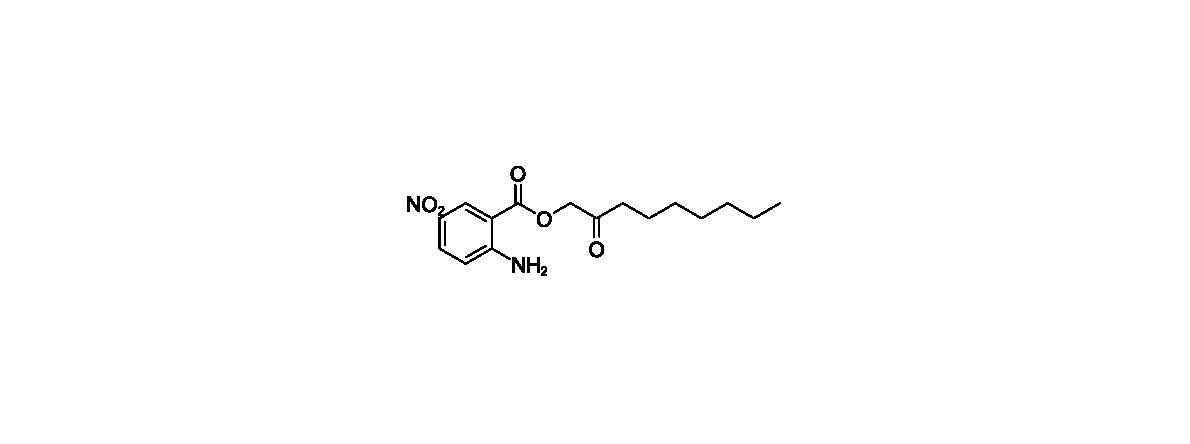
\includegraphics[scale=1]{5Naae}
	\end{center}
\end{scheme}

%LMO-1-039
%LMO-1-041

5-Nitroanthranilic acid \compound{cmpd:5naa} (500 mg, 2.75 mmol, 1.38 eq.) and potassium carbonate (270 mg, 2.00 mmol, 1 eq.) were dissolved in DMF (5 mL). The mixture was heated under argon to $90\ ^{\circ}$C and stirred for 1 h then cooled to r.t.. 1-Chlorononan-2-one \compound{cmpd:Clnon} (353 mg, 2.00 mmol, 1 eq.) was added and the mixture was stirred for 15 h. The solution was poured into \ce{Na2HCO3} (aq., 10\%, 50 mL) and ice (\textasciitilde ~20 g). The precipitate was collected by vacuum filtration, washed with water and dried under high vacuum. \compound{cmpd:5naae} was obtained as a yellow amorphous solid (0.674 g, 2.00 mmol, 100\%).
\\[1\baselineskip]
\noindent{\textbf{mp} \textit{T} / $^{\circ}$C = 135 (water)}
%rough
\\[1\baselineskip]
\noindent{\textbf{IR} (neat) $\nu_{max}$ / cm$^{-1}$ =
	3453 (N-H),
	3351 (N-H),
	2925 (C-H),
	2854 (C-H),
	1720 (ester C=O)
	1704 (ketone C=O)
	1626 (N-H bend)
	1603 (aromatic)
	1573 (N-O)
	1507 (N-O)}
\\[1\baselineskip]
\noindent{\textbf{$^{1}$H NMR} (400 MHz, DMSO-d$_6$) $\delta$ / ppm = 
	8.66 (d, \textit{J} = 2.8 Hz, 1 H, \textit{ortho} to C(=O)), 
	8.12 (dd, \textit{J} = 2.8, 9.4 Hz, 1 H, \textit{para} to C(=O)), 
	6.93 (d, \textit{J} = 9.4 Hz, 1 H, \textit{meta} to C(=O)), 
	5.05 (s, 2 H, OC\underline{H}$_2$C(=O)),
	2.49 (t, \textit{J} = 7.4 Hz, 2 H, C(=O)C\underline{H}$_2$CH$_2$), 
	1.52 (quin, \textit{J} = 7.2 Hz, 2 H, C(=O)CH$_2$C\underline{H}$_2$), 
	1.32 - 1.20 (m, 8 H,         C\underline{H}$_2$C\underline{H}$_2$C\underline{H}$_2$C\underline{H}$_2$CH$_3$), 
	0.86 (t, \textit{J} = 6.8 Hz, 3 H, C\underline{H}$_3$)}
\\[1\baselineskip]
\noindent{\textbf{$^{13}$C NMR} (101 MHz, DMSO-d$_6$) $\delta$ / ppm = 
	204.4 (OCH$_2$\underline{C}(=O)), 
	165.6 (\underline{C}(=O)O), 
	156.3 (\textit{ipso} to NH$_2$), 
	135.7 (\textit{ipso} to NO$_2$), 
	129.6 (\textit{para} to C(=O)), 
	128.9 (\textit{ortho} to C(=O)), 
	117.4 (\textit{meta} to C(=O)), 
	107.5 (\textit{ipso} to C(=O)), 
	68.8 (O\underline{C}H$_2$C(=O)), 
	38.3 (C(=O)\underline{C}H$_2$CH$_2$), 
	31.6 (\underline{C}H$_2$CH$_2$CH$_3$), 
	28.9 (\underline{C}H$_2$), 
	28.9 (\underline{C}H$_2$), 
	23.2 (C(=O)CH$_2$\underline{C}H$_2$), 
	22.5 (\underline{C}H$_2$CH$_3$), 
	14.4 (\underline{C}H$_3$)}
\\[1\baselineskip]
\noindent{\textbf{HRMS} (ESI$^+$) \textit{m}/\textit{z} / Da = 323.1610, [M+H]$^+$, [\ce{C16H23N2O5}]$^+$ requires 323.1607}
\\[1\baselineskip]
Spectroscopic data are consistent with the literature\cite{Baker2015}.

\subsection{6-Nitro-2-heptyl-3-hydroxyquinolin-4(1\textit{H})-one \compound{cmpd:NPQS}}

%Yssynov
%LMO-1-045

\begin{scheme}[H]
	\begin{center}
		\includegraphics[scale=1]{NPQS}
	\end{center}
\end{scheme}

2-Oxononyl 2-amino-5-nitrobenzoate \compound{cmpd:5naae} (100 mg, 0.340 mmol, 1 eq.) and polyphosphoric acid (300 mg) were stirred for 5.5 h at $90\ ^{\circ}$C under argon. The mixture was then poured into \ce{NaHCO3} (sat., aq., 50 mL) cooled on ice. The precipitate was collected by vacuum filtration, washed with water (50 mL) and dried under high vacuum. \compound{cmpd:NPQS} was obtained as a yellow-brown amorphous solid (44 mg, 0.145 mmol, 43\%).% which could be recrystallised from EtOAc to give yellow-brown plate-like crystals.
\\[1\baselineskip]
\noindent{\textbf{mp} \textit{T} / $^{\circ}$C = 223 (water, EtOAc)}
%rough
\\[1\baselineskip]
\noindent{\textbf{IR} (neat) $\nu_{max}$ / cm$^{-1}$ =
	3436 (N-H),
	3000 (O-H, br),
	2955 (C-H),
	2926 (C-H),
	2851 (C-H),
	1648 (C=O),
	%1606 (aromatic),
	1571 (N-O),
	1536 (N-O)}
\\[1\baselineskip]
\noindent{\textbf{$^{1}$H NMR} (400 MHz, DMSO-d$_6$) $\delta$ / ppm = 
	12.00 (s, 1 H, N\underline{H}), 
	8.91 (d, \textit{J} = 2.8 Hz, 1 H, \textit{ortho} to C=O), 
	8.29 (dd, \textit{J} = 2.7, 9.2 Hz, 1 H, \textit{para} to C=O), 
	7.70 (d, \textit{J} = 9.3 Hz, 1 H, \textit{meta} to C=O), 
	2.75 (t, \textit{J} = 7.7 Hz, 2 H, CC\underline{H}$_2$), 
	1.67 (quin, \textit{J} = 7.3 Hz, 2 H, CCH$_2$C\underline{H}$_2$), 
	1.36 - 1.23 (m, 8 H, C\underline{H}$_2$C\underline{H}$_2$C\underline{H}$_2$C\underline{H}$_2$CH$_3$), 
	0.85 (t, \textit{J} = 7.0 Hz, 3 H, C\underline{H}$_3$)}
\\[1\baselineskip]
\noindent{\textbf{$^{13}$C NMR} (101 MHz, DMSO-d$_6$) $\delta$ / ppm = 
	169.7 (\underline{C}=O), 
	141.9 (\textit{para} to NO$_2$), 
	140.7 (\textit{ipso} to NO$_2$), 
	139.6 (\textit{ipso} to OH), 
	137.3 (\underline{C}=COH), 
	124.3 (\textit{para} to C=O), 
	122.3 (\textit{ortho} to NO$_2$ and \textit{ortho} to C=O), 
	121.5 (\textit{ipso} to C=O),
	120.0 (\textit{meta} to NO$_2$ and \textit{meta} to C=O), 
	31.6 (\underline{C}H$_2$CH$_2$CH$_3$), 
	29.2 (\underline{C}H$_2$), 
	28.9 (\underline{C}H$_2$), 
	28.5 (C\underline{C}H$_2$), 
	28.1 (CCH$_2$\underline{C}H$_2$), 
	22.5 (\underline{C}H$_2$CH$_3$), 
	14.4 (\underline{C}H$_3$)}
\\[1\baselineskip]
\noindent{\textbf{HRMS} (ESI$^+$) \textit{m}/\textit{z} / Da = 305.1501, [M+H]$^+$, [\ce{C16H21N2O4}]$^+$ requires 305.1500}
\\[1\baselineskip]
Spectroscopic data are consistent with the literature\cite{Baker2015}.

\subsection{6-Amino-2-heptyl-3-hydroxyquinolin-4(1\textit{H})-one \compound{cmpd:amPQS}}


%LMO-1-044 (NMR empty),LMO-1-048, LMO-1-053
%Yssynov


\begin{scheme}[H]
	\begin{center}
		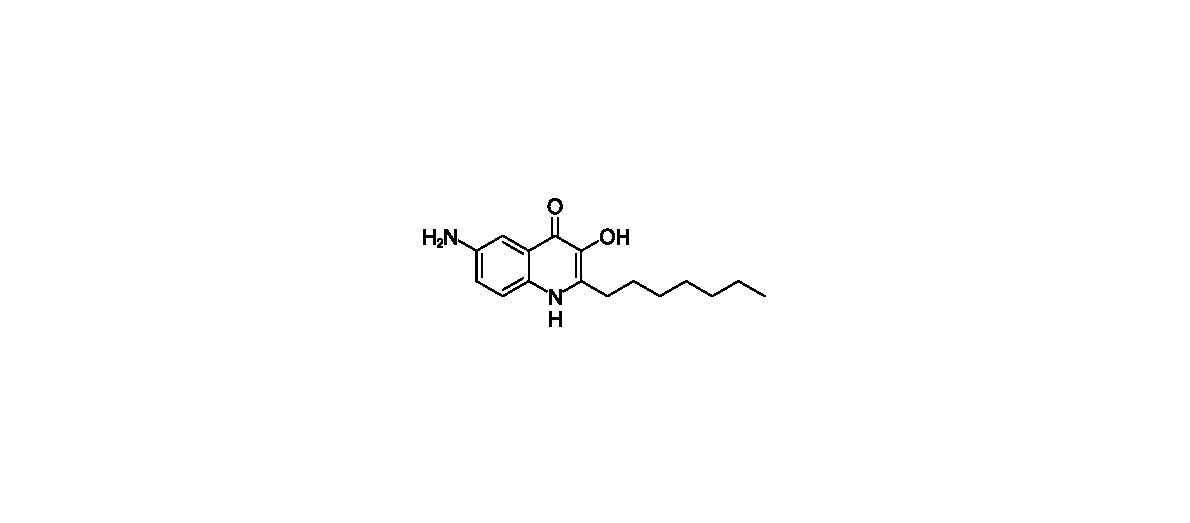
\includegraphics[scale=1]{amPQS}
	\end{center}
\end{scheme}

6-Nitro-2-heptyl-3-hydroxyquinolin-4(1\textit{H})-one \compound{cmpd:NPQS} (20 mg, 0.0658 mmol, 1 eq.) and \ce{PtO2} (2 mg, 10 weight \%) were stirred in MeOH (1 mL) under a \ce{H2} atmosphere for 45 min at room temperature and pressure. The reaction mixture was then filtered through celite and the solvent was removed under vacuum. \compound{cmpd:amPQS} was obtained as a yellow-brown amorphous solid (14.5 mg, 0.0529 mmol, 80\%).
\\[1\baselineskip]
\noindent{\textbf{mp} (\ce{MeOH}) \textit{T} / $^{\circ}$C = 176}
%rough
\\[1\baselineskip]
\noindent{\textbf{IR} (neat) $\nu_{max}$ / cm$^{-1}$ =
	30000 (O-H, br)
	29251 (C-H),
	28549 (C-H), 
	16133 (C=O)}
	%15559 (aromatic)
	%15047 (aromatic)}
\\[1\baselineskip]
\noindent{\textbf{$^{1}$H NMR} (400 MHz, MeOD) $\delta$ / ppm = 
	11.12 (s, 1 H, N\underline{H}), 
	7.47 (d, \textit{J} = 8.9 Hz, 1 H, \textit{meta} to C=O), 
	7.40 (d, \textit{J} = 2.4 Hz, 1 H, \textit{ortho} to C=O), 
	7.16 (dd, \textit{J} = 2.6, 9.0 Hz, 1 H, \textit{para} to C=O), 
	2.86 (t, \textit{J} = 7.5 Hz, 2 H, CC\underline{H}$_2$), 
	1.75 (quin, \textit{J} = 7.8 Hz, 2 H, CCH$_2$C\underline{H}$_2$), 
	1.48 - 1.22 (m, \textit{J} = 5.4 Hz, 8 H, C\underline{H}$_2$C\underline{H}$_2$C\underline{H}$_2$C\underline{H}$_2$CH$_3$), 
	0.89 (t, \textit{J} = 6.7 Hz, 3 H, C\underline{H}$_3$)}
\\[1\baselineskip]
\noindent{\textbf{$^{13}$C NMR} (101 MHz, MeOD) $\delta$ / ppm = 
	166.8 (\underline{C}(=O)), 
	144.8 (\textit{para} to NH$_2$ or \textit{ipso} to C(=O)), 
	140.5 (\underline{C}OH), 
	138.6 (\underline{C}=COH), 
	132.6 (\textit{ipso} to NH$_2$), 
	124.8 (\textit{para} to NH$_2$ or \textit{ipso} to C(=O)), 
	123.8 (\textit{para} to C(=O)), 
	107.7 (\textit{meta} to NH$_2$ and \textit{meta} to C(=O)), 
	106.4 (\textit{ortho} to NH$_2$ and \textit{ortho} to C(=O)), 
	33.0 (\underline{C}H$_2$CH$_2$CH$_3$), 
	29.5 - 31.0 (C\underline{C}H$_2$\underline{C}H$_2$\underline{C}H$_2$\underline{C}H$_2$), 
	23.8 (\underline{C}H$_2$CH$_3$), 
	14.5 (\underline{C}H$_3$)}
\\[1\baselineskip]
\noindent{\textbf{HRMS} (ESI$^+$) \textit{m}/\textit{z} / Da = 275.1760, [M+H]$^+$, [\ce{C16H23N2O2}]$^+$ requires 275.1762}
\\[1\baselineskip]
Spectroscopic data are not consistent with the literature\cite{Baker2015}. It is possible that Baker's product is a Zn adduct.% as her $^{13}$C NMR value for the carbon \textit{ipso} to NH$_2$ is rather high\cite{Darque2009}.

\subsection{6-Azido-2-heptyl-3-hydroxyquinolin-4(1\textit{H})-one \compound{cmpd:azPQS}}

%LMO-2-046(precip empty, something in other), LMO-1-056



\begin{scheme}[H]
	\begin{center}
		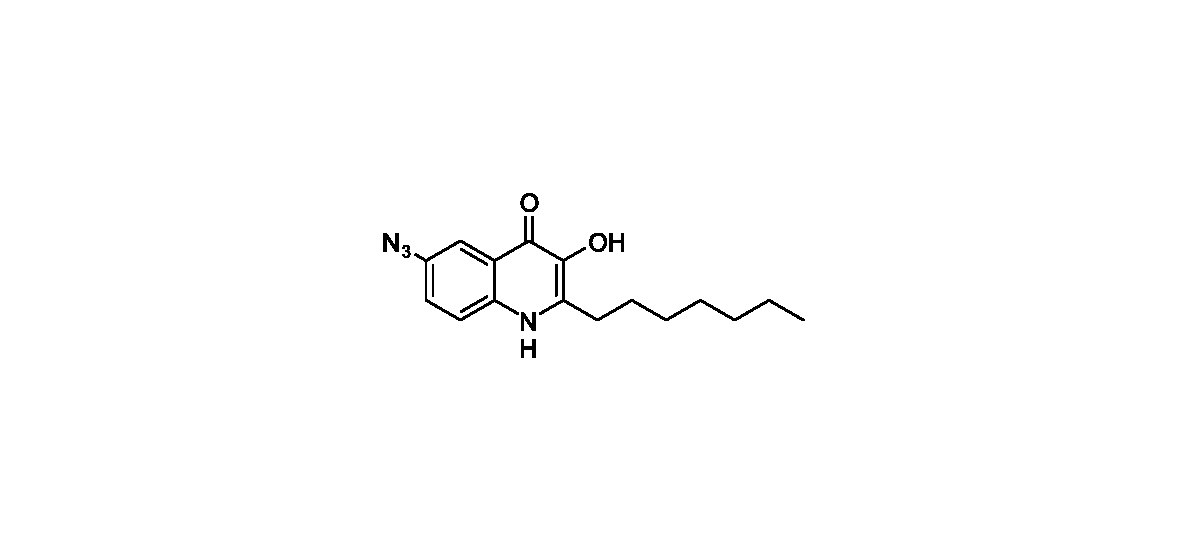
\includegraphics[scale=1]{azPQS}
	\end{center}
\end{scheme}

6-Amino-2-heptyl-3-hydroxyquinolin-4(1\textit{H})-one \compound{cmpd:amPQS} (18.2 mg, 0.0664 mmol, 1 eq.) was dissolved in HCl (conc., aq., 0.8 mL) and MeOH (0.5 mL) at 0 $^{\circ}$C. \ce{NaNO2} (5.0 mg, 0.0725 mmol, 1.09 eq.) in water (0.2 mL) was added dropwise over 2 min and the mixture was stirred at 0 $^{\circ}$C for 50 min, during which time the solution turned from yellow to orange. \ce{NaN3} (4.9 mg, 0.0754 mmol, 1.14 eq.) in water (0.2 mL) was then added and the mixture was allowed to warm to r.t. and stirred for 4 h. The reaction mixture was then filtered and the solid was dried under reduced pressure. \compound{cmpd:azPQS} was obtained as a brown amorphous solid (5.5 mg, 0.0183 mmol, 28\%).
\\[1\baselineskip]
\noindent{\textbf{IR} (neat) $\nu_{max}$ / cm$^{-1}$ = 
	3089 (N-H), 
	2921 (C-H), 
	2851 (C-H), 
	2108 (azide), 
	1632 (C=O)}
\\[1\baselineskip]
\noindent{\textbf{$^{1}$H NMR} (400 MHz, DMSO-d$_6$) $\delta$ / ppm =
	7.74 (s, 1 H, \textit{ortho} to C=O), 
	7.65 (d, \textit{J} = 6.9 Hz, 1 H, \textit{meta} to C(=O)), 
	7.32 (d, \textit{J} = 7.4 Hz, 1 H, \textit{para} to C(=O)), 
	2.75 (t, \textit{J} = 7.5 Hz, 2 H, CC\underline{H}$_2$), 
	1.67 (quin, \textit{J} = 6.4 Hz, 2 H, CCH$_2$C\underline{H}$_2$), 
	1.43 - 1.13 (m, 8 H, C\underline{H}$_2$C\underline{H}$_2$C\underline{H}$_2$C\underline{H}$_2$CH$_3$), 
	0.85 (t, \textit{J} = 6.8 Hz, 3 H, C\underline{H}$_3$)}
\\[1\baselineskip]
\noindent{\textbf{$^{13}$C NMR} (101 MHz, DMSO-d$_6$) $\delta$ / ppm = 
	166.3 (\underline{C}(=O)),
	137.9 (), 
	137.8 (\underline{C}N$_3$), 
	134.5 (\textit{ipso} to C(=O)), 
	133.9 (\underline{C}=COH), 
	122.7 (\textit{para} to C(=O)), 
	122.6 (\textit{meta} to N$_3$ and \textit{meta} to C(=O)), 
	120.4 (\textit{para} to N$_3$), 
	112.4 (\textit{ortho} to N$_3$ and \textit{ortho} to C(=O)), 
	31.2 (\underline{C}H$_2$CH$_2$CH$_3$), 
	28.8 (C\underline{C}H$_2$), 
	28.4 (CCH$_2$CH$_2$\underline{C}H$_2$), 
	28.3 (CCH$_2$CH$_2$CH$_2$\underline{C}H$_2$), 
	27.8 (CCH$_2$\underline{C}H$_2$), 
	22.1 (\underline{C}H$_2$CH$_3$), 
	14.0 (\underline{C}H$_3$)
	}
\\[1\baselineskip]
\noindent{\textbf{HRMS} (ESI$^+$) \textit{m}/\textit{z} / Da = 301.1649, [M+H]$^+$, [\ce{C16H21N4O2}]$^+$ requires 301.1659}
\\[1\baselineskip]
Spectroscopic data are consistent with the literature\cite{Baker2015}.

\subsection{(\textit{S})-3-Aminodihydrofuran-2(3\textit{H})-one hydrobromide \compound{cmpd:HLHBr}}

%lit
%LMO-1-001

\begin{scheme}[H]
	\begin{center}
		\includegraphics[scale=1]{HLHBr}
	\end{center}
\end{scheme}

\textsc{l}-Methionine \compound{cmpd:LM} (3.04 g, 20.4 mmol, 1 eq.) and bromoacetic acid \compound{cmpd:HOO2Br} (3.08 g, 22.2 mmol, 1.09 eq.) were dissolved in \textit{i}-PrOH (12.5 mL), H$_2$O (12.5 mL) and AcOH (5 mL). The reaction was refluxed for 15 h then concentrated under vacuum. The resulting brown oil was added to a mixture of \textit{i}-PrOH (16 mL) and HBr (33\% in AcOH, 4 mL), causing the precipitation of a pale pink amorphous solid. The precipitate was collected by filtration and washed with \textit{i}-PrOH (20 mL). The filtrate was concentrated under vacuum and precipitated again using the same procedure. The two crops of precipitate were combined. \compound{cmpd:HLHBr} was obtained as a pale pink amorphous solid (1.73 g, 9.50 mmol, 41\% yield).
\\[1\baselineskip]
\noindent{\textbf{mp} \textit{T} / $^{\circ}$C = 242 (\textit{i}-PrOH/AcOH, gas evolved)}
%rough
\\[1\baselineskip]
\noindent{\textbf{IR} (neat) $\nu_{max}$ / cm$^{-1}$ =
	2972 (N-H),
	2878 (N-H),
	1772 (C=O),
	1585 (N-H bend),
	1572 (N-H bend)}
\\[1\baselineskip]
\noindent{\textbf{$^{1}$H NMR} (400 MHz, DMSO-d$_6$) $\delta$ / ppm = 
	8.59 (br s, 3 H, N\underline{H}$_3^+$), 
	4.46 (dt, \textit{J} = 1.3, 8.9 Hz, 1 H, OC\underline{H}H), 
	4.37 (dd, \textit{J} = 8.8, 11.4 Hz, 1 H, C\underline{H}NH$_3^+$), 
	4.29 (ddd, \textit{J} = 6.1, 8.8, 10.9 Hz, 1 H, OCH\underline{H}), 
	2.57 (dddd, \textit{J} = 1.2, 6.1, 8.9, 12.3 Hz, 1 H, OCH$_2$C\underline{H}H), 
	2.26 (dtd, \textit{J} = 9.0, 11.2, 12.2 Hz, 1 H, OCH$_2$CH\underline{H})}
\\[1\baselineskip]
\noindent{\textbf{$^{13}$C NMR} (101 MHz, DMSO-d$_6$) $\delta$ / ppm = 
	173.3 (\underline{C}=O), 
	66.2 (O\underline{C}H$_2$), 
	47.8 (\underline{C}HNH$_3^+$), 
	27.0 (OCH$_2$\underline{C}H$_2$)}
\\[1\baselineskip]
\noindent{[\bm{$\alpha$}]$_D^{20}$ / $^{\circ}$10$^{-1}$cm$^2$g$^{-1}$ = -30.0, lit. = -25.0 (\textit{c} / g(100 mL)$^{-1}$ = 0.0200, DMSO)}
\\[1\baselineskip]
The data are consistent with the literature\cite{Stacy2013}.
%Mp: 240-244 °C; 1
%H NMR (300 MHz,
%CH3OD) δ 4.89 (s, 3H), 4.53 (dt, \textit{J} = 9.1, 1.1 Hz, 1H), 4.42-4.33 (m, 2H), 2.74 (dddd, \textit{J} = 12.5, 8.9, 5.9, 1.2 Hz, 1H), 2.33 (dddd, \textit{J} = 12.5, 11.7, 11.0, 9.1 Hz, 1H); 13
%C NMR (75 MHz, DMSO-
%d6) δ 173.2, 66.3, 47.7, 26.9; \textbf{IR} (neat) cm-1
%: 2986, 2880, 1775, 1496, 1210, 1155, 1009; [α]D
%20
%: - 25.00°

\subsection{(\textit{S})-2-Bromo-\textit{N}-(2-oxotetrahydrofuran-3-yl)acetamide \compound{cmpd:HL2Br}}

%lit
%LMO-1-009

\begin{scheme}[H]
	\begin{center}
		\includegraphics[scale=1]{HL2Br}
	\end{center}
\end{scheme}

(\textit{S})-3-Aminodihydrofuran-2(3\textit{H})-one hydrobromide \compound{cmpd:HLHBr} (100 mg, 0.549 mmol, 1.08 eq.) and \ce{NaHCO3} (84.9 mg, 1.01 mmol, 2.00 eq.) were dissolved in \ce{CH2Cl2} (2 mL) and water (2 mL). Bromoacetyl bromide \compound{cmpd:Br2Br} (44.0 $\mu$L, 102 mg, 0.505 mmol, 1.00 eq.) was then added dropwise. The reaction mixture was stirred for 24 h, after which the \ce{CH2Cl2} was removed under vacuum. The aqueous phase was extracted with EtOAc (4$\times$10 mL). The combined organic layers were dried with \ce{MgSO4} and the solvent was removed under reduced pressure. \compound{cmpd:HL2Br} was obtained as white, needle-like crystals (88.0 mg, 0.396 mmol, 74\%).
\\[1\baselineskip]
\noindent{\textbf{mp} \textit{T} / $^{\circ}$C = 132 (EtOAc)}
%rough
\\[1\baselineskip]
\noindent{\textbf{IR} (neat) $\nu_{max}$ / cm$^{-1}$ =
	3256 (N-H),
	3067 (C-H),
	1763 (lactone C=O),
	1658 (amide C=O),
	1553 (N-H bend)}
\\[1\baselineskip]
\noindent{\textbf{$^{1}$H NMR} (400 MHz, \ce{CDCl3}) $\delta$ / ppm = 
	6.94 (br s, 1 H, N\underline{H}), 
	4.57 (ddd, \textit{J} = 11.7, 8.6, 5.9 Hz, 1 H, C\underline{H}NH), 
	4.51 (td, \textit{J} = 9.2, 1.0 Hz, 1 H, OC\underline{H}H), 
	4.32 (ddd, \textit{J} = 11.3, 9.4, 5.9 Hz, 1 H, OCH\underline{H}), 
	3.93 (s, 1 H, C\underline{H}HBr), 
	3.93 (s, 1 H, CH\underline{H}Br), 
	2.87 (dddd, \textit{J} = 12.6, 8.6, 5.9, 1.3 Hz, 1 H, OCH$_2$C\underline{H}H), 
	2.22 (dtd, \textit{J} = 12.6, 11.5, 11.5, 8.9 Hz, 1 H, OCH$_2$CH\underline{H})}
\\[1\baselineskip]
%lit
%δ 8.83 (d, \textit{J} = 7.7 Hz, 1H), 4.60 (dt, \textit{J} = 10.6, 8.5 Hz,
%1H), 4.36 (t, \textit{J} = 8.8 Hz, 1H), 4.21 (ddd, \textit{J} = 9.8, 9.0, 6.4 Hz, 1H), 3.92 (s, 2H), 2.47-2.38 (m, 1H), 2.22-2.08 (m, 1H)
\noindent{\textbf{$^{13}$C NMR} (101 MHz, \ce{CDCl3}) $\delta$ / ppm = 
	174.6 (O\underline{C}=O), 
	166.4 (\underline{C}(=O)NH), 
	66.1 (O\underline{C}H$_2$), 
	49.8 (\underline{C}HNHC=O), 
	29.9 (OCH$_2$\underline{C}H$_2$), 
	28.2 (O=C\underline{C}H$_2$Br)}
\\[1\baselineskip]
\noindent{\textbf{HRMS} The compound does not ionise.}
\\[1\baselineskip]
\noindent{[\bm{$\alpha$}]$_D^{20}$ / $^{\circ}$10$^{-1}$cm$^2$g$^{-1}$ = 27.0, lit. = 20.5 (\textit{c} / g(100 mL)$^{-1}$ = 0.00740, \ce{CHCl3})}
\\[1\baselineskip]
The data are consistent with the literature\cite{Stacy2013,Nielsen2005}.

%1
%H NMR (300 MHz, DMSO-d6
%) δ 8.83 (d, \textit{J} = 7.7 Hz, 1H), 4.60 (dt, \textit{J} = 10.6, 8.5 Hz, 1H), 4.36 (t, \textit{J} = 8.8 Hz, 1H), 4.21 (ddd, \textit{J} = 9.8, 9.0, 6.4 Hz, 1H), 3.92 (s, 2H), 2.47-2.38 (m, 1H), 2.22-2.08 (m, 1H); 13
%C NMR (75 MHz, DMSO-d6
%) δ 174.7, 166.1, 65.3, 48.3, 28.8, 27.9.

\subsection{(\textit{S})-2-Azido-\textit{N}-(2-oxotetrahydrofuran-3-yl)acetamide \compound{cmpd:HL2N3}}

%lit
%LMO-1-008

\begin{scheme}[H]
	\begin{center}
		\includegraphics[scale=1]{HL2N3}
	\end{center}
\end{scheme}

(3\textit{S})-2-Oxotetrahydrofuran-3-aminium bromide \compound{cmpd:HLHBr} (100 mg, 0.552 mmol, 1.08 eq.), \ce{NaN3} (85.7 mg, 1.32 mmol, 2.61 eq.) and \ce{NaHCO3} (84.9 mg, 1.01 mmol, 2.00 eq.) were dissolved in \ce{CH2Cl2} (2 mL) and water (2 mL). Bromoacetyl bromide \compound{cmpd:Br2Br} (44.0 $\mu$L, 102 mg, 0.505 mmol, 1.00 eq.) was then added dropwise. The reaction mixture was stirred for 48 h, after which the \ce{CH2Cl2} was removed under vacuum. The aqueous phase was extracted with EtOAc (4$\times$10 mL). The combined organic layers were dried with \ce{MgSO4} and the solvent was removed under reduced pressure. \compound{cmpd:HL2N3} was obtained as white, needle-like crystals (38.4 mg, 0.209 mmol, 41\%).
\\[1\baselineskip]
\noindent{\textbf{mp} \textit{T} / $^{\circ}$C = 87 (EtOAc)}
%rough
\\[1\baselineskip]
\noindent{\textbf{IR} (neat) $\nu_{max}$ / cm$^{-1}$ =
	3284 (N-H),
	2923 (C-H),
	2853 (C-H),
	2130 (\ce{N3}),
	1783 (lactone C=O),
	1661 (amide C=O),
	1537 (N-H bend)}
\\[1\baselineskip]
\noindent{\textbf{$^{1}$H NMR} (400 MHz, \ce{CDCl3}) $\delta$ / ppm = 
	7.05 (br d, \textit{J} = 6.5 Hz, 1 H, N\underline{H}), 
	4.64 (ddd, \textit{J} = 11.6, 8.7, 6.8 Hz, 1 H, C\underline{H}NH), 
	4.48 (td, \textit{J} = 9.1, 1.3 Hz, 1 H, OC\underline{H}H), 
	4.30 (ddd, \textit{J} = 11.2, 9.2, 6.0 Hz, 1 H, OCH\underline{H}), 
	4.04 (s, 2 H, C\underline{H}$_2$N$_3$), 
	2.76 (dddd, \textit{J} = 12.5, 8.8, 6.0, 1.4 Hz, 1 H, OCH$_2$C\underline{H}H), 
	2.25 (dtd, \textit{J} = 12.5, 11.4, 11.4, 8.9 Hz, 1 H, OCH$_2$CH\underline{H})}
\\[1\baselineskip]
\noindent{\textbf{$^{13}$C NMR} (101 MHz, \ce{CDCl3}) $\delta$ / ppm = 
	174.9 (O\underline{C}=O), 
	167.5 (\underline{C}=ONH), 
	66.0 (O\underline{C}H$_2$), 
	52.2 (O=C\underline{C}H$_2$N$_3$)}, 
	48.9 (\underline{C}HNHC=O),  
	29.7 (OCH$_2$\underline{C}H$_2$)
\\[1\baselineskip]
\noindent{\textbf{HRMS} The compound does not ionise.}
\\[1\baselineskip]
\noindent{[\bm{$\alpha$}]$_D^{20}$ / $^{\circ}$10$^{-1}$cm$^2$g$^{-1}$ = -32.6, lit. = -24.4 (\textit{c} / g(100 mL)$^{-1}$ = 0.0430, DMSO)}
\\[1\baselineskip]
The data are consistent with the literature\cite{Stacy2013}.

%Mp: 82-85 °C; 1
%H NMR (300 MHz, DMSO-
%d6) δ 8.66 (d, \textit{J} = 7.8 Hz, 1H) 4.60 (td, \textit{J} = 10.6, 8.5 Hz, 1H), 4.36 (dt, \textit{J} = 8.9, 1.4 Hz, 1H), 4.21 (ddd, \textit{J} = 9.8, 9.0, 6.4 Hz, 1H), 3.92 (s, 2H) 2.46-2.37 (m, 1H) 2.25-2.11 (m, 1H); 13
%C NMR (75
%MHz, DMSO-d6 ) δ 175.0, 167.6, 65.4, 50.6 48.1, 28.1; \textbf{IR} (neat) cm-1: 3281, 2111, 1778, 1660,
%
%1530, 1384, 1224, 1173, 1026 ; Rf 
%= 0.30 (ethyl acetate, vanillin); [α]D 20 : -24,4° (c: 0.043, DMSO).

\subsection{(\textit{S})-4-Bromo-\textit{N}-(2-oxotetrahydrofuran-3-yl)butanamide \compound{cmpd:HL4Br}}

%LMO-1-059

\begin{scheme}[H]
	\begin{center}
		\includegraphics[scale=1]{HL4Br}
	\end{center}
\end{scheme}

(\textit{S})-3-Aminodihydrofuran-2(3\textit{H})-one hydrobromide \compound{cmpd:HLHBr} (200 mg, 1.10 mmol, 1.00 eq.) and \ce{NaHCO3} (170 mg, 2.02 mmol, 1.84 eq.) were dissolved in \ce{CH2Cl2} (2 mL) and water (2 mL). Bromobutyryl chloride \compound{cmpd:Cl4Br} (140 $\mu$L, 224 mg, 1.21 mmol, 1.10 eq.) was then added dropwise. The reaction mixture was stirred for 1 h, after which the \ce{CH2Cl2} was removed under vacuum. The aqueous phase was extracted with EtOAc (7$\times$5 mL) and the combined organic layers were dried with \ce{MgSO4}. The solvent was removed under vacuum to give white crystals which were recrystallised from EtOAc. \compound{cmpd:HL4Br} was obtained as white, needle-like crystals (219 mg, 0.878 mmol, 80\%).
\\[1\baselineskip]
\noindent{\textbf{mp} \textit{T} / $^{\circ}$C = 105 (EtOAc)}
%rough
\\[1\baselineskip]
\noindent{\textbf{IR} (neat) $\nu_{max}$ / cm$^{-1}$ =
	3308 (N-H),
	3074 (C-H),
	2949 (C-H),
	1774 (lactone C=O),
	1644 (amide C=O),
	1541 (N-H bend)}
\\[1\baselineskip]
\noindent{\textbf{$^{1}$H NMR} (400 MHz, \ce{CDCl3}) $\delta$ / ppm = 
	6.31 (br d, \textit{J} = 5.5 Hz, 1 H, N\underline{H}), 
	4.59 (ddd, \textit{J} = 6.2, 8.7, 11.5 Hz, 1 H, C\underline{H}NH), 
	4.48 (dt, \textit{J} = 1.2, 8.9 Hz, 1 H, OC\underline{H}H), 
	4.30 (ddd, \textit{J} = 5.8, 9.3, 11.3 Hz, 1 H, OCH\underline{H}), 
	3.49 (t, \textit{J} = 6.3 Hz, 2 H, C\underline{H}$_2$Br), 
	2.82 (dddd, \textit{J} = 1.3, 5.9, 8.7, 12.5 Hz, 1 H, OCH$_2$C\underline{H}H), 
	2.47 (t, \textit{J} = 7.3 Hz, 2 H, C(=O)C\underline{H}$_2$), 
	2.26 - 2.15 (m, 3 H, OCH$_2$CH\underline{H} and C\underline{H}$_2$CH$_2$Br)}
\\[1\baselineskip]
\noindent{\textbf{$^{13}$C NMR} (101 MHz, \ce{CDCl3}) $\delta$ / ppm = 
	175.4 (O\underline{C}=O), 
	172.3 (\underline{C}(=O)NH), 
	66.1 (O\underline{C}H$_2$), 
	49.3 (\underline{C}HNHC=O), 
	33.9 (C(=O)\underline{C}H$_2$), 
	33.1 (\underline{C}H$_2$Br), 
	30.3 (OCH$_2$\underline{C}H$_2$), 
	27.9 (C(=O)CH$_2$\underline{C}H$_2$)}
\\[1\baselineskip]
\noindent{\textbf{HRMS} The compound does not ionise.}
\\[1\baselineskip]
\noindent{[\bm{$\alpha$}]$_D^{26.6}$ / $^{\circ}$10$^{-1}$cm$^2$g$^{-1}$ = -78 (\textit{c} / g(100 mL)$^{-1}$ = 0.0833, MeOH)}
\\[1\baselineskip]
The compound has not been reported previously.

%\subsection{(\textit{S})-4-azido-\textit{N}-(2-oxotetrahydrofuran-3-yl)butanamide \compound{cmpd:HL4N3}\cite{Baker2012}}

\subsection{(\textit{S})-6-Bromo-\textit{N}-(2-oxotetrahydrofuran-3-yl)hexanamide \compound{cmpd:HL6Br}}

%nov
%LMO-1-050

\begin{scheme}[H]
	\begin{center}
		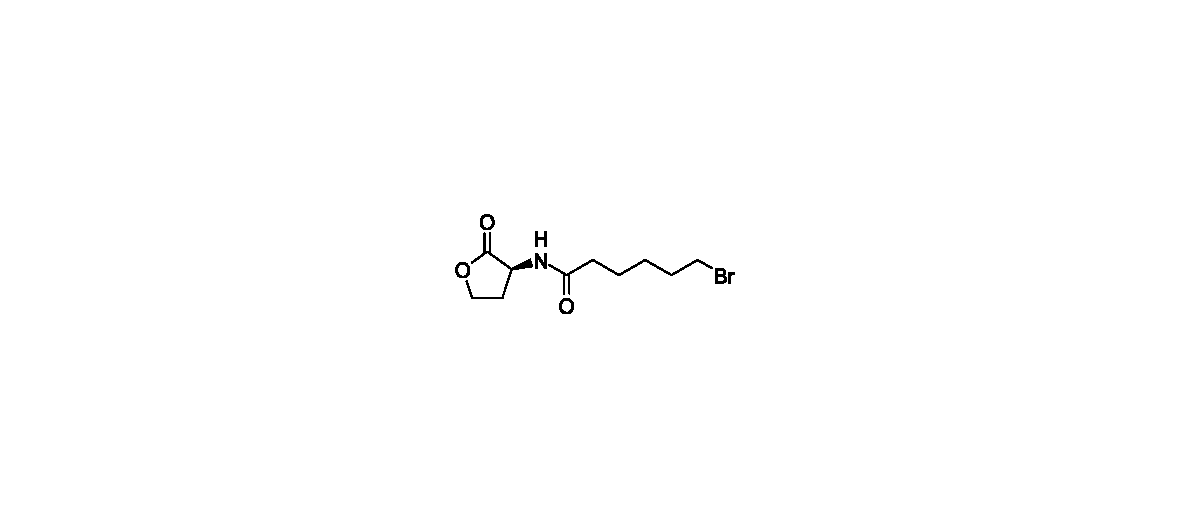
\includegraphics[scale=1]{HL6Br}
	\end{center}
\end{scheme}

(\textit{S})-3-Aminodihydrofuran-2(3\textit{H})-one hydrobromide \compound{cmpd:HLHBr} (100 mg, 0.549 mmol, 1.00 eq.) and \ce{NaHCO3} (84.9 mg, 1.01 mmol, 1.84 eq.) were dissolved in \ce{CH2Cl2} (2 mL) and water (2 mL) at r.t.. Bromohexanoyl chloride \compound{cmpd:Cl6Br} (93.0 $\mu$L, 130 mg, 0.608 mmol, 1.11 eq.) was then added dropwise. The reaction mixture was stirred for 4 h, after which the \ce{CH2Cl2} was removed under vacuum. The mixture was then filtered, washed with water (10 mL) and dried under high vacuum. \compound{cmpd:HL6Br} was obtained as white, needle-like crystals (101 mg, 0.362 mmol, 66\%).
\\[1\baselineskip]
\noindent{\textbf{mp} \textit{T} / $^{\circ}$C = 106 (\ce{CH2Cl2}, water)}
%rough
\\[1\baselineskip]
\noindent{\textbf{IR} (neat) $\nu_{max}$ / cm$^{-1}$ =
	3300 (N-H),
	3068 (C-H),
	2937 (C-H),
	2857 (C-H),
	1785 (lactone C=O),
	1639 (amide C=O),
	1540 (N-H bend)}
\\[1\baselineskip]
\noindent{\textbf{$^{1}$H NMR} (400 MHz, \ce{CDCl3}) $\delta$ / ppm = 
	6.09 (br d, \textit{J} = 5.7 Hz, 1 H, N\underline{H}), 
	4.57 (ddd, \textit{J} = 5.9, 8.6, 11.6 Hz, 1 H, C\underline{H}NH), 
	4.50 (dt, \textit{J} = 1.3, 9.1 Hz, 1 H, OC\underline{H}H), 
	4.31 (ddd, \textit{J} = 5.9, 9.3, 11.3 Hz, 1 H, OCH\underline{H}), 
	3.43 (t, \textit{J} = 6.7 Hz, 2 H, C\underline{H}$_2$Br), 
	2.88 (dddd, \textit{J} = 1.3, 5.9, 8.6, 12.6 Hz, 1 H, OCH$_2$C\underline{H}H), 
	2.30 (dt, \textit{J} = 1.8, 7.5 Hz, 2 H, C(=O)C\underline{H}$_2$), 
	2.16 (dtd, \textit{J} = 8.9, 11.5, 12.5 Hz, 1 H, OCH$_2$CH\underline{H}), 
	1.90 (quin, \textit{J} = 7.2 Hz, 2 H, C\underline{H}$_2$CH$_2$Br), 
	1.71 (quin, \textit{J} = 7.6 Hz, 2 H, C(=O)CH$_2$C\underline{H}$_2$), 
	1.59 - 1.46 (m, 2 H, C(=O)CH$_2$CH$_2$C\underline{H}$_2$)}
\\[1\baselineskip]
\noindent{\textbf{$^{13}$C NMR} (101 MHz, \ce{CDCl3}) $\delta$ / ppm = 
	175.5 (O\underline{C}=O), 
	173.3 (\underline{C}(=O)NH),  
	66.1 (O\underline{C}H$_2$), 
	49.3 (\underline{C}HNHC=O), 
	35.8 (\underline{C}H$_2$Br), 
	33.5 (C(=O)\underline{C}H$_2$), 
	32.3 (\underline{C}H$_2$CH$_2$Br), 
	30.5 (OCH$_2$\underline{C}H$_2$), 
	27.6 (C(=O)CH$_2$\underline{C}H$_2$), 
	24.4 (C(=O)CH$_2$\allowbreak CH$_2$\underline{C}H$_2$)}
\\[1\baselineskip]
\noindent{\textbf{HRMS} (ESI$^+$) \textit{m}/\textit{z} / Da = 278.0381, [M+H]$^+$, [\ce{C10H17BrNO3}]$^+$ requires 278.0386}
\\[1\baselineskip]
\noindent{[\bm{$\alpha$}]$_D^{26.6}$ / $^{\circ}$10$^{-1}$cm$^2$g$^{-1}$ = -16 (\textit{c} / g(100 mL)$^{-1}$ = 0.208, MeOH)}
\\[1\baselineskip]
The compound has not been reported previously.

\subsection{(\textit{S})-6-Azido-\textit{N}-(2-oxotetrahydrofuran-3-yl)hexanamide \compound{cmpd:HL6N3}}

\begin{scheme}[H]
	\begin{center}
		\includegraphics[scale=1]{HL6N3}
	\end{center}
\end{scheme}

(\textit{S})-6-Bromo-\textit{N}-(2-oxotetrahydrofuran-3-yl)hexanamide \compound{cmpd:HL6Br} (80 mg, 0.320 mmol, 1.00 eq.) and \ce{NaN3} (26.3 mg, 0.405 mmol, 1.27 eq.) were heated in DMF (0.5 mL) for 5 h at $100\ ^{\circ}$C. The reaction mixture was then partitioned between \ce{CH2Cl2} (5 mL) and water (5 mL). The aqueous phase was extracted twice more with \ce{CH2Cl2} (2$\times$5 mL) and the organic layers were combined and dried over \ce{MgSO4}. The solvent was removed by rotary evaporation followed by high vacuum. \compound{cmpd:HL6N3} was obtained as white, needle-like crystals (42.7 mg, 0.178 mmol, 56\%).
\\[1\baselineskip]
\noindent{\textbf{mp} \textit{T} / $^{\circ}$C = 90 (\ce{CH2Cl2})}
%rough
\\[1\baselineskip]
\noindent{\textbf{IR} (neat) $\nu_{max}$ / cm$^{-1}$ =
	3314 (N-H),
	2932 (C-H),
	2863 (C-H),
	2095 (\ce{N3}),
	1775 (lactone C=O),
	1643 (amide C=O),
	1548 (N-H bend)}
\\[1\baselineskip]
\noindent{\textbf{$^{1}$H NMR} (400 MHz, \ce{CDCl3}) $\delta$ / ppm = 
	5.96 (d, \textit{J} = 4.2 Hz, 1 H, N\underline{H}), 
	4.54 (ddd, \textit{J} = 11.7, 8.6, 5.7 Hz, 1 H, C\underline{H}NH), 
	4.49 (td, \textit{J} = 9.1, 1.0 Hz, 1 H, OC\underline{H}H), 
	4.30 (ddd, \textit{J} = 11.3, 9.4, 5.8 Hz, 1 H, OCH\underline{H}), 
	3.29 (t, \textit{J} = 6.9 Hz, 2 H, C\underline{H}$_2$N$_3$), 
	2.88 (dddd, \textit{J} = 12.5, 8.6, 5.8, 1.1 Hz, 1 H, OCH$_2$C\underline{H}H), 
	2.28 (t, \textit{J} = 7.5 Hz, 1 H, C(=O)C\underline{H}H), 
	2.28 (t, \textit{J} = 7.4 Hz, 1 H, C(=O)CH\underline{H}),
	2.14 (dtd, \textit{J} = 12.3, 11.5, 11.5, 8.8 Hz, 1 H, OCH$_2$C\underline{H}H), 
	1.70 (quin, \textit{J} = 7.6 Hz, 2 H, C\underline{H}$_2$CH$_2$N$_3$), 
	1.63 (quin, \textit{J} = 7.2 Hz, 2 H, C(=O)CH$_2$C\underline{H}$_2$), 
	1.38 - 1.49 (m, 2 H, C(=O)CH$_2$CH$_2$C\underline{H}$_2$)}
\\[1\baselineskip]
\noindent{\textbf{$^{13}$C NMR} (101 MHz, \ce{CDCl3}) $\delta$ / ppm = 
	175.4 (O\underline{C}=O), 
	172.2 (\underline{C}(=O)NH), 
	66.1 (O\underline{C}H$_2$), 
	51.2 (\underline{C}H$_2$N$_3$), 
	49.4 (\underline{C}HNHC=O), 
	35.9 (C(=O)\underline{C}H$_2$), 
	30.7 (OCH$_2$\underline{C}H$_2$), 
	28.6 (\underline{C}H$_2$CH$_2$N$_3$), 
	26.3 (C(=O)CH$_2$\underline{C}H$_2$), 
	24.8 (C(=O)CH$_2$\allowbreak CH$_2$\underline{C}H$_2$)}
\\[1\baselineskip]
\noindent{\textbf{HRMS} (ESI$^+$) \textit{m}/\textit{z} / Da = 241.1289, [M+H]$^+$, [\ce{C10H17N4O3}]$^+$ requires 241.1295}
\\[1\baselineskip]
\noindent{[\bm{$\alpha$}]$_D^{26.6}$ / $^{\circ}$10$^{-1}$cm$^2$g$^{-1}$ = -16 (\textit{c} / g(100 mL)$^{-1}$ = 0.208, MeOH)}
\\[1\baselineskip]
The compound has not been reported previously.

\subsection{Hex-5-ynal \compound{cmpd:hexynal}}

%lit
%LMO-1-014
%LMO-1-015
%LMO-1-023

\begin{scheme}[H]
	\begin{center}
		\includegraphics[scale=1]{hexynal}
	\end{center}
\end{scheme}

Pyridinium chlorochromate (14.6 g, 68.1 mmol, 1.50 eq) and \ce{CH2Cl2} (500 mL) were stirred at r.t. under argon. 5-Hexyn-1-ol \compound{cmpd:hexynol} (5.00 mL, 45.4 mmol, 1 eq.) was added and the reaction mixture was stirred for 5 h followed by addition of \ce{Et2O} (125 mL) and silica gel (62.5 g). The suspension was stirred for 1 h then filtered through a pad of silica (100 g) and washed with \ce{Et2O}. The solvent was removed by rotary evaporation. \compound{cmpd:hexynal} was obtained as a pale yellow-green oil (4.72 g, 49.1 mmol, 72\%).
\\[1\baselineskip]
\noindent{\textbf{IR} (neat) $\nu_{max}$ / cm$^{-1}$ =
	3293 (alkyne C-H),
	2943 (alkane C-H),
	2831 (aldehyde C-H),
	2729 (aldehyde C-H),
	1720 (aldehyde C=O)}
\\[1\baselineskip]
\noindent{\textbf{$^{1}$H NMR} (400 MHz, \ce{CDCl3}) $\delta$ / ppm = 
	9.80 (s, 1 H, C(=O)\underline{H}), 
	2.60 (t, \textit{J} = 7.1 Hz, 2 H, C\underline{H}$_2$C(=O)H), 
	2.26 (dt, \textit{J} = 2.6, 6.8 Hz, 2 H, HC$\equiv$CC\underline{H}$_2$), 
	1.98 (t, \textit{J} = 2.7 Hz, 1 H, \underline{H}C$\equiv$C), 
	1.85 (quin, \textit{J} = 7.0 Hz, 2 H, HC$\equiv$CCH$_2$C\underline{H}$_2$)}
\\[1\baselineskip]
\noindent{\textbf{$^{13}$C NMR} (101 MHz, \ce{CDCl3}) $\delta$ / ppm = 
	201.6 (\underline{C}(=O)), 
	83.1 (HC$\equiv$\underline{C}), 
	69.3 (H\underline{C}$\equiv$C), 
	42.4 (\underline{C}H$_2$C(=O)), 
	20.7 (\underline{C}H$_2$CH$_2$C(=O)), 
	17.6 (HC$\equiv$C\underline{C}H$_2$)}
\\[1\baselineskip]
Spectroscopic data are consistent with the literature\cite{Kocsis2012}.

%(300 MHz, CDCl3) 9.82 (t, \textit{J} = 1.2 Hz, 1H), 2.62 (dt, \textit{J} = 1.2, 7.2 Hz, 2H), 2.28 (dt, \textit{J} = 2.4, 6.8 Hz, 2H), 1.99 (t, \textit{J} = 2.4 Hz, 1H), 1.87 (p, \textit{J} = 7.1 Hz, 2H) ppm

\subsection{\textit{tert}-Butyl 4-(hex-5-yn-1-yl)piperazine-1-carboxylate \compound{cmpd:hexpipboc}}

%nov
%LMO-1-016
%LMO-1-018
%LMO-1-063

\begin{scheme}[H]
	\begin{center}
		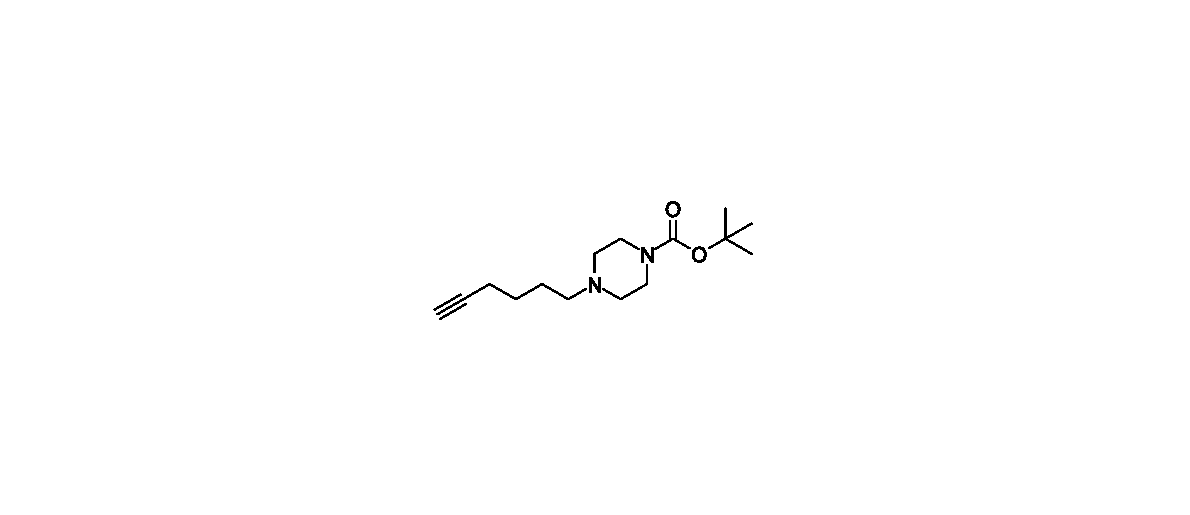
\includegraphics[scale=1]{hexpipboc}
	\end{center}
\end{scheme}

Hex-5-ynal \compound{cmpd:hexynal} (0.407 g, 4.24  mmol, 1.00 eq.) and \textit{tert}-butyl piperazine-1-carboxylate \compound{cmpd:pipboc} (0.791 g, 4.24 mmol, 1.00 eq.) were stirred under a \ce{N2} atmosphere in 1,2-dichloro\-ethane (20 mL) for 2.5 h followed by addition of sodium triacetoxyborohydride (6.25 g, 29.5 mmol, 7 eq.) in four portions over 4 d. The mixture was stirred for a further day then \ce{NaHCO3} (sat., aq., 120 mL) was added and the product extracted with EtOAc (2$\times$100 mL). The solvent was dried over \ce{MgSO4} and removed by rotary evaporation. \compound{cmpd:hexpipboc} was obtained as a colourless liquid (1.12 g, 4.21 mmol, 99\%).
\\[1\baselineskip]
\noindent{\textbf{TLC} \textit{R$_f$} (10\% MeOH/\ce{CH2Cl2}) = 0.55}
\\[1\baselineskip]
\noindent{\textbf{IR} (neat) $\nu_{max}$ / cm$^{-1}$ =
	3304 (alkyne C-H),
	2940 (alkane C-H),
	2865 (C-H),
	2810 (C-H),
	1691 (carbamate C=O)}
\\[1\baselineskip]
\noindent{\textbf{$^{1}$H NMR} (400 MHz, \ce{CDCl3}) $\delta$ / ppm = 
	3.44 (t, \textit{J} = 5.2 Hz, 4 H, CH$_2$CH$_2$CH$_2$N(CH$_2$C\underline{H}$_2$)CH$_2$C\underline{H}$_2$), 
	2.39 (t, \textit{J} = 5.1 Hz, 4 H, CH$_2$CH$_2$CH$_2$N(C\underline{H}$_2$)C\underline{H}$_2$), 
	2.37 (t, \textit{J} = 7.3 Hz, 2 H, CH$_2$CH$_2$C\underline{H}$_2$N), 
	2.23 (dt, \textit{J} = 2.7, 6.8 Hz, 2 H, HC$\equiv$CC\underline{H}$_2$), 
	1.96 (t, \textit{J} = 2.7 Hz, 1 H, \underline{H}C$\equiv$C), 
	1.65 - 1.53 (m, 4 H,            HC$\equiv$CCH$_2$C\underline{H}$_2$C\underline{H}$_2$), 
	1.47 (s, 9 H, C\underline{H}$_3$)}
\\[1\baselineskip]
\noindent{\textbf{$^{13}$C NMR} (101 MHz, \ce{CDCl3}) $\delta$ / ppm = 
	154.7 (N\underline{C}(=O)O), 
	84.2 (HC$\equiv$\underline{C}), 
	79.6 (\underline{C}(CH$_3$)$_3$), 
	68.5 (H\underline{C}$\equiv$C), 
	60.4 (CH$_2$CH$_2$\underline{C}H$_2$N), 
	58.0 (CH$_2$CH$_2$CH$_2$N(\underline{C}H$_2$)\underline{C}H$_2$), 
	53.0 (CH$_2$CH$_2$CH$_2$N(CH$_2$\underline{C}H$_2$)CH$_2$\underline{C}H$_2$),
	28.4 (C(\underline{C}H$_3$)$_3$), 
	26.3 (\underline{C}H$_2$CH$_2$N), 
	25.7 (HC$\equiv$CCH$_2$\underline{C}H$_2$), 
	18.3 (HC$\equiv$C\underline{C}H$_2$)}
\\[1\baselineskip]
\noindent{\textbf{HRMS} (ESI$^+$) \textit{m}/\textit{z} / Da = 267.2073, [M+H]$^+$, [\ce{C15H27N2O2}]$^+$ requires 267.2064}
\\[1\baselineskip]
The compound has not been reported previously.

% tail amine not hex
%13C NMR (CDCl3, 50 MHz): ä
%154.9, 79.7, 58.5, 53.1, 43.7, 41.8, 31.1, 28.5, 24.2

\subsection{1-(Hex-5-yn-1-yl)piperazine \compound{cmpd:hexpip}}

%nov
%LMO-1-017
%LMO-1-020

\begin{scheme}[H]
	\begin{center}
		\includegraphics[scale=1]{hexpip}
	\end{center}
\end{scheme}

\textit{tert}-Butyl 4-(hex-5-yn-1-yl)piperazine-1-carboxylate \compound{cmpd:hexpipboc} (763 mg, 2.86 mmol) was stirred in TFA (10 mL) at r.t. for 2 h. The TFA was removed under vacuum followed by co-evaporation with \ce{CH2Cl2} (2$\times$20 mL). The oil was diluted with water (10 mL) and the pH adjusted to 14 with NaOH (10\% aq.). This mixture was extracted with \ce{CH2Cl2} (2$\times$20 mL) and the combined organic layers were dried over \ce{MgSO4}. The solvent was removed under vacuum and purified by column chromatography (\ce{SiO2} MeOH/\ce{CH2Cl2} 3:7). \compound{cmpd:hexpip} was obtained as a colourless liquid (476 mg, 2.86 mmol, 100\%).
\\[1\baselineskip]
\noindent{\textbf{TLC} \textit{R$_f$} (30\% MeOH/\ce{CH2Cl2}) = 0.20}
\\[1\baselineskip]
\noindent{\textbf{IR} (neat) $\nu_{max}$ / cm$^{-1}$ =
	3296 (alkyne C-H),
	2941 (alkane C-H),
	2811 (alkane C-H),
	1637 (N-H bend)}
\\[1\baselineskip]
\noindent{\textbf{$^{1}$H NMR} (400 MHz, \ce{CDCl3}) $\delta$ / ppm = 
	2.88 (t, \textit{J} = 4.9 Hz, 4 H, CH$_2$CH$_2$CH$_2$N(CH$_2$C\underline{H}$_2$)CH$_2$C\underline{H}$_2$), 
	2.39 (m, 4 H, CH$_2$CH$_2$CH$_2$N(C\underline{H}$_2$)C\underline{H}$_2$), 
	2.31 (t, \textit{J} = 7.1 Hz, 2 H, HC$\equiv$CCH$_2$CH$_2$CH$_2$C\underline{H}$_2$N), 
	2.20 (dt, \textit{J} = 2.7, 6.8 Hz, 2 H, HC$\equiv$CC\underline{H}$_2$), 
	2.05 (br s, 1 H, N\underline{H}), 
	1.93 (t, \textit{J} = 2.7 Hz, 1 H, \underline{H}C$\equiv$C), 
	1.65 - 1.48 (m, 4 H, HC$\equiv$CCH$_2$C\underline{H}$_2$C\underline{H}$_2$\-CH$_2$N)}
\\[1\baselineskip]
\noindent{\textbf{$^{13}$C NMR} (101 MHz, \ce{CDCl3}) $\delta$ / ppm = 
	84.3 (HC$\equiv$\underline{C}), 
	68.4 (H\underline{C}$\equiv$C), 
	58.6 (CH$_2$CH$_2$\underline{C}H$_2$N), 
	54.5 (CH$_2$CH$_2$\allowbreak CH$_2$N(\underline{C}H$_2$)\underline{C}H$_2$), 
	46.0 (CH$_2$CH$_2$CH$_2$N(CH$_2$\underline{C}H$_2$)CH$_2$\underline{C}H$_2$), 
	26.4 (CH$_2$\underline{C}H$_2$CH$_2$N), 
	25.7 (HC$\equiv$CCH$_2$\underline{C}H$_2$), 
	18.3 (HC$\equiv$C\underline{C}H$_2$)}
\\[1\baselineskip]
\noindent{\textbf{HRMS} (ESI$^+$) \textit{m}/\textit{z} / Da = 167.1548, [M+H]$^+$, [\ce{C10H19N2}]$^+$ requires 167.1548}
\\[1\baselineskip]
The compound has not been reported previously.

\subsection{1-Cyclopropyl-6-fluoro-7-(4-(hex-5-yn-1-yl)piperazin-1-yl)-4-oxo-1,4\hyp{}dihydro\-quinoline-3-carboxylic acid \compound{cmpd:Y4Cip}}

%%nov
%%LMO-1-019
%%LMO-1-021
%%LMO-1-065
%%LMO-1-066
%%LMO-1-089

\begin{scheme}[H]
	\begin{center}
		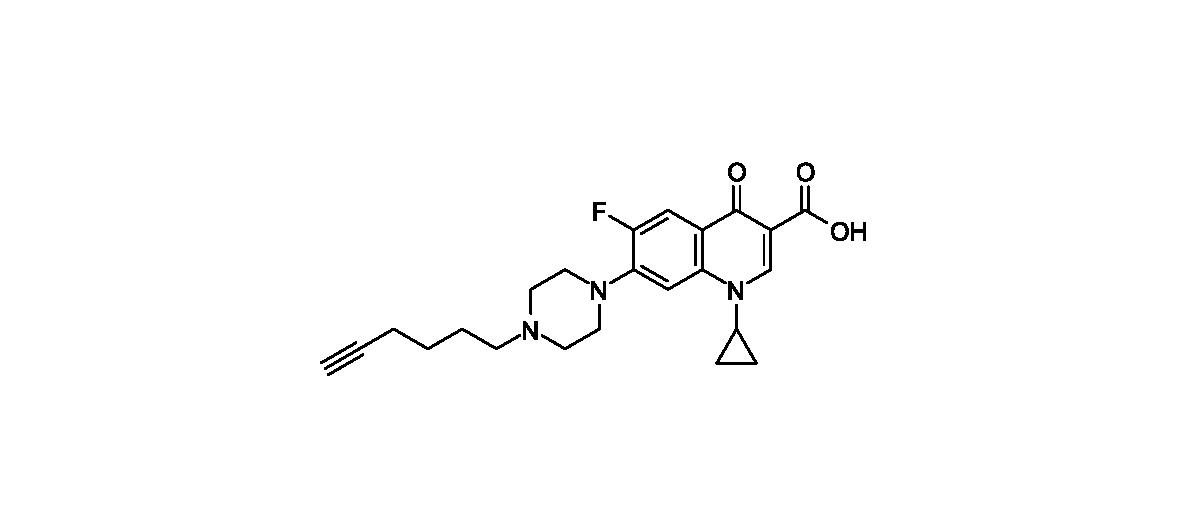
\includegraphics[scale=1]{Y4Cip}
	\end{center}
\end{scheme}

7-Chloro-1-cyclopropyl-6-fluoro-4-oxo-1,4-dihydroquino\hyp{}line-3-carboxylic acid \compound{cmpd:Clcip} (1.27 g, 4.51 mmol, 1 eq.), 1-(hex-5-yn-1-yl)piperazine \compound{cmpd:hexpip} (1.5 g, 9.02 mmol, 2 eq.) and \textit{N}-methyl-2-pyrrolidone (10 mL) were stirred in a microwave reactor at 115 $^{\circ}$C for 24 h. The reaction mixture was cooled to r.t. and water (80 mL) was added. The mixture was stirred for 3 h and then filtered, and residue was washed with MeOH (50 mL). The resulting solid (0.571 g) was further purified by recrystalisation from EtOAc (50 mL). \compound{cmpd:Y4Cip} was obtained as off-white crystals (0.219 g, 0.531 mmol, 12\%).
\\[1\baselineskip]
\noindent{\textbf{TLC} \textit{R$_f$} = 0.02 (10\% MeOH/\ce{CH2Cl2})}
\\[1\baselineskip]
\noindent{\textbf{mp} \textit{T} / $^{\circ}$C = 220 (MeOH, decomposes)}
%rough
\\[1\baselineskip]
\noindent{\textbf{IR} (neat) $\nu_{max}$ / cm$^{-1}$ =
	3212 (alkyne C-H),
	2459 (O-H),
	1723 (carboxylic acid C=O),
	1627 (quinolone C=O)}
\\[1\baselineskip]
\noindent{\textbf{$^{1}$H NMR} (500 MHz, DMSO-d$_6$) $\delta$ / ppm = 
	15.12 (br s, 1 H, C(=O)O\underline{H}), 
	8.69 (s, 1 H, \textit{ortho} to C(=O)OH), 
	7.96 (d, \textit{J} = 13.0 Hz, 1 H, \textit{ortho} to F), 
	7.61 (d, \textit{J} = 7.6 Hz, 1 H, \textit{meta} to F), 
	3.82 - 3.92 (m, 3 H, NC\underline{H}(CH$_2$)$_2$ and CH$_2$CH$_2$CH$_2$N(CH$_2$C\underline{H}$_2$)CH$_2$CH$_2$), 
	3.54 - 3.68 (br m, 2 H, CH$_2$CH$_2$CH$_2$N(C\underline{H}$_2$)CH$_2$), 
	3.45 (br. t, \textit{J} = 11.6 Hz, 2 H, CH$_2$CH$_2$CH$_2$N(CH$_2$CH$_2$)CH$_2$C\underline{H}$_2$), 
	3.21 - 3.29 (br m, 2 H, CH$_2$CH$_2$CH$_2$N(CH$_2$CH$_2$)CH$_2$C\underline{H}$_2$), 
	3.11 - 3.20 (br m, 2 H, CH$_2$CH$_2$CH$_2$N(CH$_2$)C\underline{H}$_2$), 
	2.84 (t, \textit{J} = 2.7 Hz, 1 H, \underline{H}C$\equiv$C), 
	2.24 (td, \textit{J} = 7.0, 2.7 Hz, 2 H, HC$\equiv$CC\underline{H}$_2$), 
	1.83 (br. quin, \textit{J} = 7.5 Hz, 2 H, HC$\equiv$CCH$_2$CH$_2$C\underline{H}$_2$), 
	1.52 (quin, \textit{J} = 7.4 Hz, 2 H, HC$\equiv$CCH$_2$C\underline{H}$_2$), 
	1.29 - 1.36 (m, 2 H, NCH(C\underline{H}H)$_2$), 
	1.16 - 1.23 (m, 2 H, NCH(CH\underline{H})$_2$)}
\\[1\baselineskip]
\noindent{\textbf{$^{13}$C NMR} (126 MHz, DMSO-d$_6$) $\delta$ / ppm = 
	176.4 (\underline{C}(=O)CC(=O)OH), 
	165.8 (\underline{C}(=O)OH), 
	152.8 (d, \textit{J} = 248.5 Hz, \textit{ipso} to F), 
	148.2 (\underline{C}HCC(=O)OH), 
	143.7 (d, \textit{J} = 11.1 Hz, \textit{para} to C(=O)), 
	139.1 (\textit{para} to F), 
	119.4 (d, \textit{J} = 6.9 Hz, \textit{ipso} to C(=O)), 
	111.2 (d, \textit{J} = 22.5 Hz, \textit{ortho} to F and \textit{ortho} to C(=O)), 
	106.9 (\textit{meta} to F and \textit{meta} to C(=O)), 
	106.9 (C(=O)\underline{C}C(=O)OH), 
	83.9 (HC$\equiv$\underline{C}), 
	71.8 (H\underline{C}$\equiv$C), 
	55.0 (CH$_2$CH$_2$\underline{C}H$_2$N), 
	50.5 (CH$_2$CH$_2$CH$_2$N(\underline{C}H$_2$)\underline{C}H$_2$), 
	46.3 (CH$_2$CH$_2$CH$_2$N(CH$_2$\underline{C}H$_2$)CH$_2$\underline{C}H$_2$), 
	36.0 (N\underline{C}H(CH$_2$)$_2$), 
	25.2 (HC$\equiv$CCH$_2$\underline{C}H$_2$), 
	22.3 (HC$\equiv$CCH$_2$CH$_2$\underline{C}H$_2$), 
	17.4 (HC$\equiv$C\underline{C}H$_2$), 
	7.6 (NCH(\underline{C}H$_2$)$_2$)}
\\[1\baselineskip]
\noindent{\textbf{$^{19}$F NMR} (376.45 MHz, MeOD) $\delta$ / ppm = 
	-121.8 (s, ciprofloxacin F)}
\\[1\baselineskip]
\noindent{\textbf{HRMS} (ESI$^+$) \textit{m}/\textit{z} / Da = 412.2036, [M+H]$^+$, [\ce{C23H27N3O3F}]$^+$ requires 412.2030}
\\[1\baselineskip]
The compound has not been reported previously.
